% Restore modern floats after loading the original institutional class.
\makeatletter\let\KavachOriginalFloat\@xfloat\makeatother
\documentclass[a4paper,12pt]{nitathesis}
\makeatletter\let\@xfloat\KavachOriginalFloat\makeatother
\usepackage[T1]{fontenc}
\usepackage[utf8]{inputenc}
\usepackage{graphicx,times,amsmath,amssymb}
\usepackage[Sonny]{fncychap}
\usepackage{booktabs,tabularx,longtable,array}
\usepackage{tikz}
\usetikzlibrary{arrows.meta,positioning}
\usepackage{listings}
\usepackage[hidelinks,breaklinks,hypertexnames=false]{hyperref}
\usepackage{etoolbox}
% Report details confirmed by the candidate in PDF review comments.
\newcommand{\ReportTitle}{KAVACH: User Login Analysis Using LLM}
\newcommand{\CandidateName}{Umakant Yadav}
\newcommand{\RollNumber}{24MCA026}
\newcommand{\DegreeName}{Master of Computer Applications}
\newcommand{\DegreeShort}{MCA}
\newcommand{\SupervisorName}{Dr. Ranjita Das}
\newcommand{\SupervisorDesignation}{Assistant Professor}
\newcommand{\HodName}{Dr. Ashim Saha}
\newcommand{\HodDesignation}{Associate Professor}
\newcommand{\SubmissionDate}{November, 2026}

\hypersetup{pdftitle={\ReportTitle},pdfauthor={\CandidateName},pdfsubject={MCA project report}}
\makeatletter
\patchcmd{\@makechapterhead}{\vspace*{50\p@}}{\vspace*{0\p@}}{}{}
\patchcmd{\@makeschapterhead}{\vspace*{50\p@}}{\vspace*{0\p@}}{}{}
\makeatother
\setlength{\headheight}{15pt}
\setlength{\parskip}{7pt}
\setlength{\emergencystretch}{3em}
\widowpenalty=10000\clubpenalty=10000
\numberwithin{figure}{chapter}
\renewcommand{\headrulewidth}{0.5pt}
\renewcommand{\footrulewidth}{0.5pt}
\fancyhf{}\fancyhead[RO,LE]{\small\nouppercase{\leftmark}}\fancyfoot[C]{\thepage}
\renewcommand{\chaptermark}[1]{\markboth{\thechapter. #1}{}}
\newcolumntype{Y}{>{\raggedright\arraybackslash}X}
\lstset{basicstyle=\ttfamily\footnotesize,breaklines=true,columns=fullflexible,keepspaces=true,frame=single,showstringspaces=false}
\definecolor{KBlue}{HTML}{164E87}
\definecolor{KTeal}{HTML}{087F8C}
\definecolor{KPurple}{HTML}{7041A5}
\definecolor{KAmber}{HTML}{9A6500}
\definecolor{KRed}{HTML}{B33D59}
\definecolor{KGray}{HTML}{526174}
\tikzset{box/.style={draw=KBlue,fill=KBlue!7,rounded corners=2pt,align=center,text width=4.2cm,minimum height=1.1cm,font=\small},flow/.style={-{Latex[length=2.5mm]},thick,draw=KBlue}}
% Editable vector diagram styles. No raster artwork is used.
\tikzset{
 dbase/.style={draw,line width=.7pt,rounded corners=2pt,align=center,inner sep=7pt,minimum height=1.05cm,font=\small},
 person/.style={dbase,draw=KGray,fill=KGray!9},
 app/.style={dbase,draw=KBlue,fill=KBlue!9},
 store/.style={dbase,draw=KTeal,fill=KTeal!9,rounded corners=0pt},
 ai/.style={dbase,draw=KPurple,fill=KPurple!9},
 check/.style={dbase,draw=KAmber,fill=KAmber!10},
 alert/.style={dbase,draw=KRed,fill=KRed!8},
 note/.style={dbase,draw=KGray!65,fill=KGray!4,font=\footnotesize},
 dep/.style={-{Latex[length=2.1mm]},draw=KBlue,line width=.8pt},
 ret/.style={dep,dashed},
 assoc/.style={draw=KGray,line width=.7pt},
 edge/.style={font=\scriptsize,align=center,fill=white,inner sep=2pt,text=black},
 boundary/.style={draw=KGray!70,dashed,rounded corners=3pt,line width=.7pt}
}
\newcommand{\dn}[6]{\node[#1,text width=#5cm] (#2) at (#3,#4) {#6};}
\newcommand{\legendline}{\par\noindent{\footnotesize\textcolor{KBlue}{Blue: application}\quad\textcolor{KTeal}{Teal: data}\quad\textcolor{KPurple}{Purple: AI}\quad\textcolor{KAmber}{Amber: decisions}\quad\textcolor{KGray}{Gray: actors / boundaries}}\par}
\newcommand{\actor}[4]{%
 \begin{scope}[shift={(#2,#3)},draw=KGray,line width=.9pt]
 \draw[fill=KGray!8] (0,.43) circle (.18);
 \draw (0,.25)--(0,-.28) (-.3,.03)--(.3,.03) (0,-.28)--(-.27,-.63) (0,-.28)--(.27,-.63);
 \coordinate (#1) at (0,0);
 \node[font=\small,align=center,text width=2.5cm] at (0,1.1) {#4};
 \end{scope}}

\newcommand{\code}[1]{\nolinkurl{#1}}
\newcommand{\fronttitle}[1]{\clearpage\thispagestyle{plain}\begin{center}\LARGE\bfseries #1\end{center}\vspace{1.2cm}}
\newcommand{\facultyblock}[3]{\begin{minipage}[t]{0.46\textwidth}\centering\rule{6cm}{0.4pt}\\#1\\#2\\#3\\\small Computer Science and Engineering\\NIT Agartala\end{minipage}}
\begin{document}
\pagenumbering{roman}\pagestyle{plain}
\begin{titlepage}\centering
{\LARGE\bfseries\MakeUppercase{\ReportTitle}\par}
\vspace{2.2cm}
\includegraphics[width=4.4cm]{images/nita_logo.png}\par
\vspace{1.5cm}{\large\bfseries\DegreeName\ Project Report\par}
\vspace{0.8cm}{\large\bfseries\CandidateName\ (\RollNumber)\par}\vfill
{\bfseries COMPUTER SCIENCE \& ENGINEERING DEPARTMENT\\NATIONAL INSTITUTE OF TECHNOLOGY, AGARTALA\\INDIA--799046\par}
\vspace{0.6cm}{\bfseries\SubmissionDate\par}\end{titlepage}
\begin{titlepage}\centering
{\LARGE\bfseries\MakeUppercase{\ReportTitle}\par}\vspace{0.8cm}
{\bfseries\itshape Report submitted to\\National Institute of Technology, Agartala\\for the award of the degree of\\\large\DegreeName\par}\vspace{0.5cm}
{\bfseries\itshape by\\\CandidateName\ (\RollNumber)\par}\vspace{0.7cm}
{\bfseries\itshape Under the Guidance of\\\SupervisorName\\\SupervisorDesignation\par}
\vspace{0.7cm}
\includegraphics[width=4cm]{images/nita_logo.png}\par\vfill
{\bfseries COMPUTER SCIENCE \& ENGINEERING DEPARTMENT\\NATIONAL INSTITUTE OF TECHNOLOGY AGARTALA\par}
\vspace{0.4cm}{\bfseries\SubmissionDate\par}\end{titlepage}
\setcounter{page}{3}
\fronttitle{Dedicated To}
\begin{center}\begin{minipage}{0.86\textwidth}
My project supervisor, \SupervisorName, \SupervisorDesignation, CSED, NIT Agartala, for his continuous guidance, valuable insights, encouragement, and unwavering trust throughout this journey. I also extend my gratitude to all faculty members of the department whose teachings and support have shaped my professional growth and helped me reach this milestone. This dedication is also extended to everyone who contributed in any way to the development of this project and supported me along the way.
\end{minipage}\end{center}
\fronttitle{REPORT APPROVAL FOR \DegreeShort}
This report entitled ``\ReportTitle'', submitted by \CandidateName\ (\RollNumber), is presented in partial fulfilment of the requirements for the award of the \textbf{\DegreeName} degree at the National Institute of Technology, Agartala.
\vspace{2.5cm}\par\noindent
\facultyblock{\SupervisorName}{(Project Supervisor)}{\SupervisorDesignation}\hfill\facultyblock{\HodName}{(Head of the Department)}{\HodDesignation}
\vspace{2cm}\par\noindent Date: \rule{5cm}{0.4pt}\\Place: NIT Agartala
\fronttitle{DECLARATION}
I declare that the work presented in this report titled ``\ReportTitle'', submitted to the Department of Computer Science and Engineering, National Institute of Technology, Agartala, for the award of the \DegreeName\ degree, represents my work and that sources used in preparing the report have been acknowledged. I understand the requirements of academic honesty and integrity and the need to avoid fabrication of results, data, or references.

This declaration is to be reviewed and signed by the candidate before submission.
\vspace{2cm}\par\hfill\begin{minipage}{7cm}\centering\rule{6cm}{0.4pt}\\\CandidateName\\\RollNumber\end{minipage}
\vspace{1.2cm}\par\noindent\SubmissionDate\\NIT Agartala
\fronttitle{CERTIFICATE}
The report titled ``\ReportTitle'', submitted by \CandidateName\ (\RollNumber), is presented for certification of the project work carried out under the guidance of the project supervisor towards the \DegreeName\ degree.

Certification and approval are subject to review and signature by the supervisor and the department.
\vspace{2.5cm}\par\noindent
\facultyblock{\SupervisorName}{(Project Supervisor)}{\SupervisorDesignation}\hfill\facultyblock{\HodName}{(Head of the Department)}{\HodDesignation}
\vspace{2cm}\par\noindent Date: \rule{5cm}{0.4pt}\\Place: NIT Agartala
\prefacesection{Acknowledgement}
I express my gratitude to my project supervisor, \SupervisorName, \SupervisorDesignation, for guidance, feedback, and encouragement during the development of KAVACH. I thank \HodName, \HodDesignation\ and Head of the Department, and the faculty of the Department of Computer Science and Engineering, National Institute of Technology Agartala, for their academic support.

I acknowledge the developers and maintainers of the open-source technologies used in this project, including Spring Boot, Spring Security, React, PostgreSQL, and supporting libraries. Their work provided the foundation for exploring authentication monitoring, rule-based anomaly detection, and tool-assisted security analysis. I also thank my family and friends for their patience and support.
\vspace{1cm}\par\hfill\CandidateName\ (\RollNumber)
\clearpage\begingroup\setlength{\parskip}{0pt}\setstretch{1.05}\listoffigures\endgroup\clearpage\begingroup\setlength{\parskip}{0pt}\setstretch{1.05}\listoftables\endgroup
\prefacesection{Abstract}
KAVACH is a web application for monitoring authentication activity, detecting rule-based login anomalies, and supporting security investigation through an AI tool interface. The implementation separates a React frontend from a Java 21 Spring Boot backend and uses PostgreSQL through Spring Data JPA. Authentication uses BCrypt password verification and bearer JSON Web Tokens; administrative operations and selected user-specific resources are protected through role and ownership checks.

The detection pipeline evaluates six conditions: failed login, unusual login time, login involving an inactive account, a previously unseen IP address, a previously unseen device string, and repeated failures within a ten-minute window. Each anomaly has a fixed severity and weight. User risk is calculated from anomaly weights recorded during the preceding 24 hours and capped at 100. Dashboard services combine login statistics, severity totals, recent critical anomalies, and a ranked user watchlist.

The AI component includes structured anomaly explanations and a two-loop orchestration service. An inner loop performs bounded model/planner and tool cycles; an outer loop processes supplied follow-up requests. Thirteen registered tools expose investigative queries and selected account or telemetry operations. A deterministic fallback supports operation when live inference is unavailable. This report documents the implementation, diagrams its data flow, explains detection rules, and presents a reproducible validation plan. It distinguishes source-confirmed behavior from proposed improvements and makes no measured accuracy, throughput, or production-readiness claims.

\noindent\textbf{Keywords:} authentication telemetry, anomaly detection, risk scoring, Spring Security, two-loop agent, security dashboard.
\clearpage\begingroup\setlength{\parskip}{0pt}\setstretch{1.05}\tableofcontents\endgroup
\clearpage\pagenumbering{arabic}\pagestyle{fancy}\raggedbottom
\chapter{Introduction}
\section{Project Overview}
Authentication records are useful evidence for investigating account misuse. A record can show whether an attempt succeeded, which account was involved, when the attempt occurred, and the associated network and client information. Individually, these events can be difficult to interpret. Grouping them with account state and recent history provides a more useful basis for investigation.

KAVACH combines login telemetry, deterministic anomaly detection, risk summaries, audit records, and an AI-assisted investigation interface in one web application. Its name refers to a shield. The project is implemented as a Spring Boot REST backend and a React single-page frontend. PostgreSQL stores the application entities. Implementation descriptions in this report refer to the supplied source snapshot \cite{repo}.

The application supports ADMIN and USER roles. Administrators can inspect organization-wide information and manage accounts through designated endpoints. Ordinary users can access selected views of their own activity. AI agent roles describe investigative and operational behavior; these are distinct from the authenticated user's security role.

\section{Problem Statement}
A basic login implementation can reject incorrect credentials without providing enough context for later investigation. A log viewer may display records without explaining their relationship to account risk. KAVACH addresses the problem of connecting authentication events to understandable alerts, recent account risk, and an investigation workflow within a small, inspectable application.

The project asks how a login event can be evaluated using explicit rules, how alerts can be summarized into a bounded user score, and how a conversational tool interface can retrieve relevant application information. The current work implements these capabilities while leaving statistical validation and deployment hardening as further work.

\section{Objectives}
\begin{enumerate}
\item Implement registration and authentication with encoded passwords and bearer tokens.
\item Persist login activity and evaluate six explicit detection rules.
\item Present anomalies, risk, trends, account status, and audit events through role-aware pages.
\item Support structured AI explanations with a deterministic fallback.
\item Implement bounded tool calling and continuation through supplied follow-ups.
\item Document the architecture and the tests needed to establish correctness and security.
\end{enumerate}

\section{System Block Diagram}
Figure~\ref{fig:architecture} summarizes implementation boundaries. The browser communicates with the backend rather than directly with PostgreSQL or the model provider. Services coordinate persistence, rule evaluation, and AI interactions.
\begin{figure}[htbp]\centering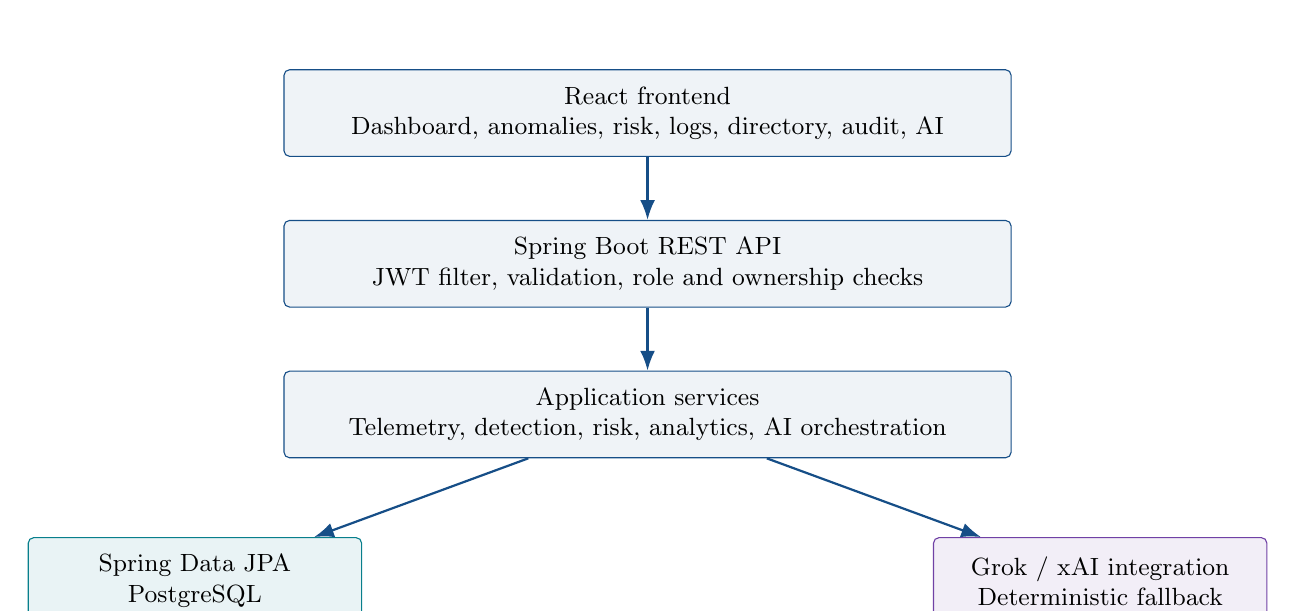
\begin{tikzpicture}[node distance=0.8cm]
\node[box,text width=9cm] (ui) {React frontend\\Dashboard, anomalies, risk, logs, directory, audit, AI};
\node[box,below=of ui,text width=9cm] (api) {Spring Boot REST API\\JWT filter, validation, role and ownership checks};
\node[box,below=of api,text width=9cm] (svc) {Application services\\Telemetry, detection, risk, analytics, AI orchestration};
\node[box,draw=KTeal,fill=KTeal!9,below left=1cm and -1cm of svc,text width=4cm] (db) {Spring Data JPA\\PostgreSQL};
\node[box,draw=KPurple,fill=KPurple!9,below right=1cm and -1cm of svc,text width=4cm] (ai) {Grok / xAI integration\\Deterministic fallback};
\draw[flow](ui)--(api);\draw[flow](api)--(svc);\draw[flow](svc)--(db);\draw[flow](svc)--(ai);
\end{tikzpicture}\caption{KAVACH implementation architecture.}\label{fig:architecture}\end{figure}

\section{Scope and Boundaries}
The project is an application-level monitoring prototype. Its rule engine does not train a machine-learning model. IP addresses are compared with stored history; no external reputation lookup is implemented. The device rule compares supplied strings, including user-agent information on the authentication path; it is not a cryptographically verified device identity.

An inactive-user alert concerns the account active flag, not elapsed account dormancy. Quarantine refers to setting an account inactive, affecting later authentication and JWT checks. It does not imply operating-system isolation or firewall enforcement.

No production traffic dataset, benchmark run, or labelled evaluation corpus was supplied. Performance and detection-accuracy claims are excluded. Chapter 5 includes source descriptions and selected candidate-provided application screenshots.

\section{Organization of the Report}
Chapters 2--4 cover requirements, design, and implementation. Chapter 5 presents interfaces, screenshots, and validation. Chapter 6 concludes with future work. Appendices document project structure, database tables, APIs, publications, and biography.
\chapter{Requirement Analysis}
\section{Software Requirements}
Table~\ref{tab:stack} lists declarations in the project manifests. Versions describe this repository rather than recommendations about current releases. Installation and execution require separate validation in the target environment.
\begin{table}[htbp]\centering\small\caption{Declared software stack.}\label{tab:stack}
\begin{tabularx}{\textwidth}{lY}\toprule Component & Declaration or purpose\\\midrule
Java & Version 21 in Maven properties.\\
Spring Boot & Parent 4.1.1; web MVC, validation, JPA, and security starters.\\
PostgreSQL & Runtime JDBC driver and relational persistence.\\
JWT & JJWT modules, version 0.12.6.\\
AI client & OpenAI Java SDK 4.101.0 used for Grok integration.\\
React & React and React DOM declared as \code{^19.3.1}.\\
Vite & Build dependency declared as \code{^8.3.6}.\\
Presentation & Tailwind CSS \code{^3.4.17}, Recharts, Lucide React, GSAP.\\
HTTP / routing & Axios and React Router DOM.\\\bottomrule\end{tabularx}\end{table}

The backend provides Maven wrapper scripts. The frontend defines development, build, preview, and Oxlint scripts. Vite uses port 5173 and forwards \code{/api} to \code{http://localhost:8080}. The Axios client supports a configurable base URL and otherwise uses \code{/api}.

\section{Functional Requirements}
\subsection{Authentication and Accounts}
Registration shall validate data, reject duplicate usernames and email addresses, encode passwords, and create active ordinary-user accounts by default. Login shall check account existence, active state, and password validity. Successful login shall return a token and safe account details. Failed and blocked requests shall produce appropriate errors and audit events.

Administrative operations shall support account inspection, creation, and active-state changes. Changes shall affect later authenticated requests because the JWT filter checks the current account record.

\subsection{Telemetry and Detection}
The system shall store timestamp, account, outcome, IP address, device, and location for login events. Authentication shall attempt to record successful and failed events for known users. The administrative ingestion path shall allow explicit event creation for controlled demonstrations.

The detector shall evaluate six independent rules. One event may create several anomalies. Before saving an anomaly, the system shall check whether the user, rule, and login record already have a matching entry.

\subsection{Risk and Analytics}
Risk shall aggregate weights of anomalies detected in the last 24 hours, cap the score at 100, and map it to four named levels. Organization-wide views shall include severity totals, risky-account totals, login outcomes, a seven-day trend, and a ranked watchlist of at most ten accounts.

\subsection{AI and Tool Operations}
The system shall provide anomaly explanations, user analysis, security summaries, history, chat, and agent-loop execution. The agent response shall include steps and tool outputs for the browser. Deterministic planning or advisory fallback shall support demonstrations when live inference is unavailable.

Tools shall expose names, argument schemas, role assignments, and parallel-safety metadata. Because some tools change accounts or create telemetry, authorization requirements must apply to the execution boundary as well as the visible page.

\section{Non-Functional Requirements}
\begin{table}[htbp]\centering\small\caption{Quality requirements and available evidence.}
\begin{tabularx}{\textwidth}{lYY}\toprule Attribute & Intended requirement & Evidence / validation needed\\\midrule
Security & Restrict protected data and actions. & JWT filter and method checks exist; tool-path policy needs explicit tests.\\
Explainability & State why alerts were generated. & Stored rule type, description, severity, and weight.\\
Maintainability & Separate presentation and business logic. & Pages, controllers, services, repositories, entities, and DTOs.\\
Reliability & Preserve failed-login telemetry. & New transaction on authentication recording; errors caught by caller.\\
Usability & Provide clear navigation and failures. & Shared UI, route guards, themes, normalized API errors.\\
Performance & Bound query and AI work. & Pagination and six inner iterations; load tests pending.\\\bottomrule\end{tabularx}\end{table}

These are requirements and implementation observations, not benchmark results. A database audit table does not establish tamper resistance, and bearer authentication does not prove every object-level access check is correct.

\section{Execution Environment and Assumptions}
Development requires Java 21, a Node.js environment compatible with the frontend dependencies, and PostgreSQL. Live inference requires provider configuration and network access. Credentials should be supplied through the existing configuration mechanisms; none are included in this report.

No measured minimum hardware specification is available. Hardware and concurrency requirements must be established by testing rather than assigning unsupported RAM or CPU figures. Timestamp rules use \code{LocalDateTime} and require a consistent time convention. Administrators must distinguish synthetic events from genuine login attempts, and AI confidence labels must not be interpreted as calibrated attack probabilities.
\chapter{Design Analysis}
\section{Layered Design}
Controllers receive HTTP requests, apply declared access restrictions, and pass inputs to services. Services implement authentication, telemetry, detection, scoring, analysis, and orchestration. Repository interfaces express persistence operations and aggregate queries. DTOs shape responses so clients receive page data without directly controlling entity persistence.

The frontend organizes features as pages and shared layout/UI components. Authentication and theme contexts hold browser state. A common Axios client adds bearer credentials, normalizes failures, and emits diagnostic information. These boundaries make the workflows traceable to source modules \cite{repo}.

% Each diagram has a dedicated page with a consistent readable vector layout.
\newsavebox{\KDiagramRaw}
\newsavebox{\KDiagramScaled}
\newcommand{\diagramview}[4]{%
\clearpage\section{#1}
#2
\legendline
\begin{figure}[!ht]\centering
\sbox{\KDiagramRaw}{\input{diagrams/#3}}
\ifdim\wd\KDiagramRaw>\textwidth
 \sbox{\KDiagramScaled}{\resizebox{\textwidth}{!}{\usebox{\KDiagramRaw}}}
\else\sbox{\KDiagramScaled}{\usebox{\KDiagramRaw}}\fi
\ifdim\dimexpr\ht\KDiagramScaled+\dp\KDiagramScaled\relax>16cm
 \resizebox*{!}{16cm}{\usebox{\KDiagramScaled}}
\else\usebox{\KDiagramScaled}\fi
\caption{#4}\end{figure}}

\diagramview{C4 Level 1: System Context}{The context view identifies the people who use KAVACH and its optional external model dependency. It treats the frontend, backend, and database as one software system. Personal and administrative scopes are distinct even though both use the same browser interface.}{c4-context}{C4 system context: actors, KAVACH, and optional model provider.}

\diagramview{C4 Level 2: Containers}{The container view decomposes KAVACH into the React application, the Spring Boot application, and PostgreSQL. Here a container means an independently executing application or data store, not a claim that Docker deployment exists. The localhost proxy reflects the supplied Vite configuration.}{c4-containers}{C4 containers: browser application, backend application, database, and provider.}

\diagramview{C4 Level 3: Backend Components}{This view expands the backend container into security, controllers, domain services, AI services, and repositories. Arrows express dependencies rather than a promise that every request follows every branch. Registry tools can bypass controller entry points, so tool execution requires its own authorization boundary.}{c4-components}{C4 backend components and external dependencies.}

\diagramview{UML Component Architecture}{The UML component view emphasizes execution environments and required interfaces. Dashed arrows denote usage dependencies. The domain-service grouping includes identity, monitoring, risk, and audit responsibilities; the AI grouping contains advisory analysis, orchestration, and operational tools.}{uml-architecture}{UML component architecture with execution boundaries and required interfaces.}

\diagramview{UML Sequence: Authentication and Detection}{Time advances down the lifelines. Solid arrows are calls and dashed arrows are responses. Known accounts produce telemetry attempts for success, bad password, or inactive-account outcomes; unknown usernames generate an audit failure without a user-linked login event. The detector may persist several anomalies per event.}{sequence-login}{UML login sequence: credentials, audit, telemetry, rules, and response.}

\diagramview{UML Sequence: Two-Loop Investigation}{The outer combined fragment represents continuation through supplied follow-ups. Its inner fragment limits model/planner cycles to six per invocation. Tool calls are sequential and feed their results into the conversation. The tool registry can reach services and repositories; live inference is optional.}{sequence-agent}{UML agent sequence: request-local queues, bounded planning, tools, and trace.}

\diagramview{Entity-Relationship Diagram}{The entity view lists mapped fields, identifiers, required links, and multiplicities. A user has zero or more login records and anomalies. Each anomaly has one required user and login event. AI history can reference either entity optionally. Audit username and cached identifiers are stored values rather than declared foreign keys.}{entity}{Detailed entity model with keys, fields, optional links, and multiplicities.}

\diagramview{UML Use-Case Diagram}{The diagram separates ordinary account capabilities from administrative capabilities. Administrator specialization inherits ordinary authenticated use cases. The model provider is a supporting external actor, not a human administrator. Associations describe intended application scope and do not certify that every agent tool enforces equivalent restrictions.}{use-cases}{UML use cases: personal investigation, administration, and optional AI support.}

\diagramview{DFD Level 0: Context}{Level 0 contains one process and three external entities: account user, administrator, and optional model provider. Its labelled flows show request and response data crossing the system boundary. Internal database stores are deliberately omitted at this level.}{dfd0}{DFD level 0: balanced context inputs and outputs.}

\diagramview{DFD Level 1: Processes and Stores}{The context process expands into identity/accounts, telemetry, detection, risk/analytics, AI investigation, and audit review. Store identifiers D1--D5 name the five entity groups. Repeated E1/E2 actors and D2/D3 stores are aliases, not additional users or databases. Query-driven risk reads do not imply automatic risk execution after detection.}{dfd1}{DFD level 1: six logical processes, five data-store groups, and external flows.}

\diagramview{DFD Level 2: Anomaly Detection}{Process 3.0 is decomposed into dispatch, six independent rule evaluations, and duplicate-aware persistence. Solid paths carry events or triggered candidates; dashed paths carry history and existence-query feedback. For new IP/device, the first event establishes a baseline. The failure-count predicate has no explicit event-time upper bound.}{dfd2-detection}{DFD level 2 of process 3.0: six rules, historical reads, and anomaly persistence.}

\diagramview{DFD Level 2: AI Investigation}{Process 5.0 separates dedicated advisory analysis from agent execution. Only the dedicated analysis path shown here explicitly stores structured analysis history. The agent path records an execution trace in its response and can invoke queries or state-changing tools. Cross-account and action permissions must be enforced before each tool invocation.}{dfd2-ai}{DFD level 2 of process 5.0: advisory analysis, model/planner, tools, and outputs.}

\clearpage\section{Database Constraints and Time Semantics}
Username and email columns are unique. Login-event indexes cover user ID, time, status, and IP address. Anomaly detection timestamps differ from login timestamps: risk uses detection time, while brute-force counting uses login time. Inserting historical events therefore requires careful interpretation.

The anomaly existence check uses user ID, rule type, and login-event ID. It prevents repeated sequential insertion but does not establish a database-level uniqueness guarantee under concurrency. Analysis history stores summaries, explanations, indicators, recommendations, confidence, model, advisory status, and cached identifiers. The audit entity provides persistence, without a demonstrated append-only or cryptographic integrity mechanism.

\section{Diagram Interpretation and Traceability}
The C4 views describe scope and structural decomposition. UML component dependencies describe required interfaces, while sequence diagrams describe ordering within representative requests. Entity associations describe persistence links. DFD arrows describe movement of data rather than control flow; the rule-dispatch order and iteration limits are explained in Chapter 4.

Names and responsibilities are derived from the controllers, services, registry, and JPA entities listed in Appendix A. Logical groupings such as ``monitoring services'' represent several existing classes rather than additional deployed services. Colors classify responsibilities and do not imply security or trust guarantees. Proposed tool-policy hardening remains a recommendation, not an implemented control.


\section{Access-Control Design}
HTTP security permits authentication routes and requires authentication elsewhere. The JWT filter validates tokens, resolves current accounts, rejects inactive users, and installs the current role. Method security is enabled. Spring documents method security as authorization on method invocations \cite{spring}.

Controllers restrict selected operations to ADMIN and allow ADMIN-or-USER access to selected personal resources. Ownership checks compare current user IDs with requested resource owners. Frontend guards guide navigation; backend policy remains authoritative.
\begin{table}[htbp]\centering\small\caption{Principal access boundaries.}
\begin{tabularx}{\textwidth}{YYY}\toprule Capability & Scope & Boundary\\\midrule
Registration / login & Public & Authentication routes.\\
Global dashboard / audit & Administrator & Controller role checks.\\
Personal logs / anomalies / risk & Administrator or owner & Selected controller and service ownership checks.\\
Directory changes & Administrator through direct API & Administrative controller methods.\\
Agent loop / tools & ADMIN or USER endpoint & Execution needs its own resource/action policy.\\\bottomrule\end{tabularx}\end{table}

Registry tools can access repositories and services directly. An administrative controller annotation does not automatically protect another call path that bypasses that controller. Centralized authorization at tool execution is therefore required hardening; this report does not assume identical policy enforcement across every REST and tool route.

\section{API and Error Handling}
The common client sends JSON, uses a 30-second timeout, and reads the bearer token from local storage. Unauthorized responses outside authentication routes clear stored credentials and dispatch an event to update UI state. The backend provides unauthorized/forbidden responses and structured application errors. Some security-filter audit failures are caught so the primary response can still be returned.

Agent requests may involve several model cycles and can outlast a single frontend timeout. Timeout, cancellation, retry, and idempotency need joint testing, especially for operations that change state.
\chapter{Functioning of the System}
\section{Registration and Authentication}
Registration trims the username, normalizes email, rejects duplicates, encodes the password, and creates an active USER account. It records an audit event and returns safe account fields. Login uses BCrypt password matching, which is hashing rather than reversible encryption.

Unknown usernames generate an audit event and an unauthorized response without user-linked telemetry. A known inactive account is blocked and failed telemetry is attempted. Incorrect passwords for active users also produce failed telemetry. Valid credentials produce a JWT, success audit entry, and successful login record.

JWT is a claims representation defined in RFC 7519 \cite{jwt}. The browser sends the token with later requests; the backend validates it and rechecks current account state. Browser logout clears local authentication information and should not be described as server-side token revocation.

\section{Telemetry Recording}
Authentication recording uses a \code{REQUIRES_NEW} transaction annotation, intended to preserve telemetry independently of a failing authentication transaction. It supplies defaults for missing IP, device, and location, saves the event, and invokes detection. The caller catches recording exceptions, so a telemetry failure can occur without replacing the main login response.

Explicit event creation accepts user ID, timestamp, IP, device, location, and status. This supports controlled demonstrations. A historical login time influences event-time rules, while a newly created anomaly receives its own detection time.

\section{Detection Engine}
\begin{table}[htbp]\centering\small\caption{Detection conditions and fixed weights.}\label{tab:rules}
\begin{tabularx}{\textwidth}{lYrr}\toprule Rule & Trigger & Weight & Severity\\\midrule
Failed login & Status is FAILED. & 20 & LOW\\
Unusual time & Login hour is at least 0 and less than 5. & 25 & LOW\\
Inactive user & Account active flag is false. & 80 & CRITICAL\\
New IP & More than one event and no other event has the same non-null IP. & 40 & MEDIUM\\
New device & More than one event and no other event has the same device, ignoring case. & 30 & MEDIUM\\
Brute force & Failed event with at least five failures after ten minutes before its timestamp. & 70 & HIGH\\\bottomrule\end{tabularx}\end{table}

All six rule methods run sequentially. A failed event at an unusual time may generate both corresponding anomalies; the brute-force rule can add another. Weights are constants rather than probabilities estimated from a dataset.

\subsection{Historical Baselines}
The new-IP and new-device rules read user history and exclude the current event by ID when seeking a match. They require more than one stored event, so the first event establishes a baseline without a new-IP/device alert. No lookback period is configured for these comparisons. Device matching ignores case, and failed events can also contribute baseline values.

The inactive-account rule checks a Boolean flag. It does not infer dormancy from the most recent successful login. IP comparison does not provide geolocation or reputation, and a device string is not an authenticated hardware identity.

\subsection{Time Windows and Duplicates}
For failed event time $t_e$, the repository counts failures satisfying $t_{login}>t_e-10\text{ minutes}$. No explicit upper bound $t_{login}\leq t_e$ is added. Chronological live input resembles a recent ten-minute count, but later stored events can affect backdated input.

Before insertion, the detector checks user ID, anomaly type, and login-event ID. Sequential reanalysis should avoid another matching anomaly. An existence query alone is not a demonstrated concurrency guarantee; a suitable unique constraint or locking policy would be required to establish that under racing requests.

\section{Risk Calculation}
Let $A_u(t)$ contain anomalies detected for user $u$ after $t-24$ hours, and let $w_a$ be a stored weight. The score is
\begin{equation}R_u(t)=\min\left(100,\sum_{a\in A_u(t)}w_a\right).\end{equation}
LOW is below 30; MEDIUM spans 30--59; HIGH spans 60--79; CRITICAL begins at 80. The risky-user count uses a recent sum of at least 60. The top-risk query groups anomalies by account, caps the score, sorts descending, and limits results to ten.

A failed login from an unseen IP on an unseen device can contribute $20+40+30=90$ if each condition holds. This makes the score CRITICAL. It is an arithmetic example, not an observed attack result. A score of 100 is not a 100 percent probability of compromise.

\section{Dashboard Composition}
The dashboard combines risk summary, login analytics, watchlist, and recent critical anomalies. Some counts are lifetime totals, risk uses 24 hours, and the trend uses seven days. Those horizons should remain visible when interpreting the figures. A user can enter a detailed investigation from a global count or watchlist account.

\section{Two-Loop AI Orchestration}
The agent request carries prompt, optional context, role, steering messages, and follow-ups. The service creates local conversation/step lists and queues copied from that request. The outer loop invokes an inner loop and later consumes supplied follow-ups.
\begin{figure}[htbp]\centering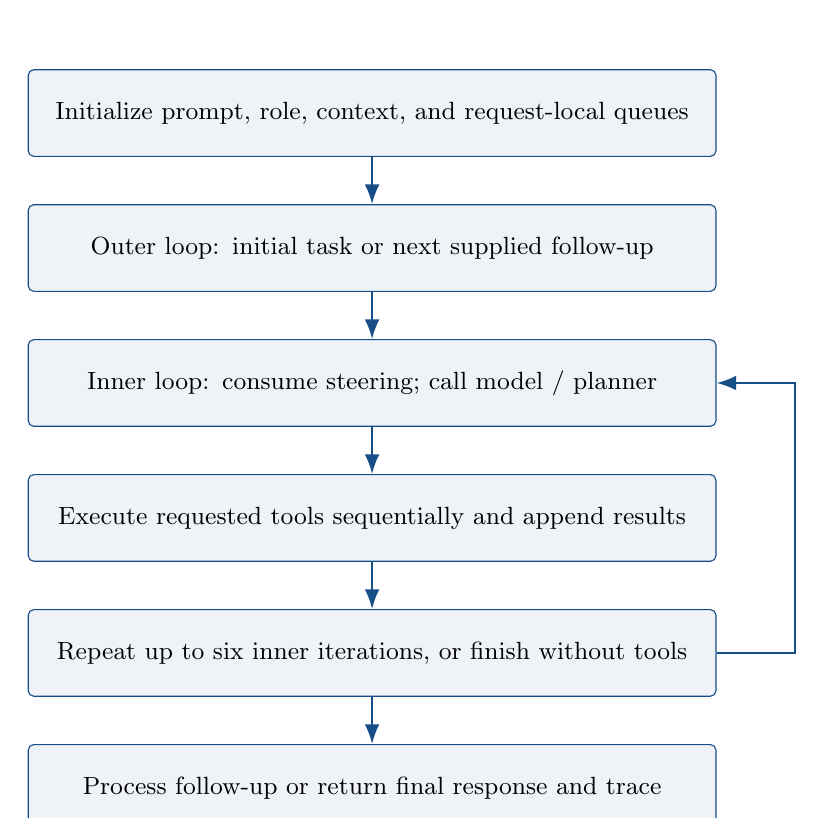
\begin{tikzpicture}[node distance=0.6cm]
\node[box,text width=8.5cm] (a) {Initialize prompt, role, context, and request-local queues};
\node[box,below=of a,text width=8.5cm] (b) {Outer loop: initial task or next supplied follow-up};
\node[box,below=of b,text width=8.5cm] (c) {Inner loop: consume steering; call model / planner};
\node[box,below=of c,text width=8.5cm] (d) {Execute requested tools sequentially and append results};
\node[box,below=of d,text width=8.5cm] (e) {Repeat up to six inner iterations, or finish without tools};
\node[box,below=of e,text width=8.5cm] (f) {Process follow-up or return final response and trace};
\foreach \x/\y in {a/b,b/c,c/d,d/e,e/f}{\draw[flow](\x)--(\y);}
\draw[flow](e.east)--++(1,0)|-(c.east);
\end{tikzpicture}\caption{Two-loop execution structure.}\label{fig:agent}\end{figure}

Before each inner iteration, at most one queued steering message enters the conversation. The model or planner returns text and optional tool calls. Each tool is resolved by name, executed, and captured as success or error output. Results enter the conversation for the next cycle. Without tool calls or pending steering, the inner loop can finish. Each invocation is capped at six iterations.

The outer loop consumes a follow-up and re-enters the inner loop until none remain. The response includes final text, execution steps, tool names, loop counts, mode, model, and completion time. Agent specializations label behavior within one service and conversation; they do not establish separately running agents.

The queues are request-local and populated at the start. No channel in this path accepts newly typed messages while execution is in progress. Current behavior supports pre-submitted steering/follow-ups; live steering is future work. Tools execute sequentially even though they advertise parallel-safety metadata.

\section{Security Tools Registry}
\begingroup\small\setstretch{1.1}\setlength{\parskip}{0pt}
\begin{longtable}{>{\raggedright\arraybackslash}p{7cm}>{\raggedright\arraybackslash}p{7.3cm}}
\caption{Thirteen registered tools.}\label{tab:tools}\\\toprule Tool & Purpose\\\midrule\endfirsthead
\toprule Tool & Purpose\\\midrule\endhead
\code{get_dashboard_security_metrics} & Combined dashboard metrics.\\
\code{list_anomalies} & Recent anomalies, optional severity and limit.\\
\code{get_anomaly_details} & Anomaly and linked login metadata.\\
\code{explain_anomaly} & Structured AI explanation.\\
\code{get_user_risk_profile} & Account's recent risk.\\
\code{get_top_risky_users} & Ranked watchlist.\\
\code{query_login_telemetry} & Login records and outcomes.\\
\code{simulate_login_event} & Insert an event and invoke detection.\\
\code{get_user_directory} & Directory information.\\
\code{update_user_account_status} & Activate or deactivate an account.\\
\code{create_directory_user} & Provision an account.\\
\code{query_audit_trail} & Audit records with optional filters.\\
\code{generate_security_summary} & AI-assisted security summary.\\\bottomrule
\end{longtable}
\endgroup

Each tool declares an argument schema, assigned role, and safety metadata. Declarations do not by themselves establish argument validation or caller authorization. Execution requires an explicit policy for principal, action, and resource. Operational tools differ from read-only explanation tools because they can change application state.

\section{Explanations, Fallback, and Audit}
Dedicated anomaly analysis checks resource access and requests JSON containing summary, explanation, indicators, implications, recommendations, and confidence. Parsing/provider failures invoke deterministic advisory output. Analysis history stores results and an advisory flag.

Action tools can update account status and save audit events. They must be assessed separately from an explanation that merely recommends action. OWASP logging guidance covers event selection, protection, and verification \cite{owasp}; these provide criteria for future work. The existing database records are not demonstrated tamper-evident logs.
\chapter{Interfaces and Validation}
\section{Documentation Method}
This chapter describes implemented pages and API relationships from source inspection and selected application screenshots provided by the candidate on 17 November 2026. The captures illustrate visible interface states; they do not establish benchmark performance or successful completion of every available action. The navigation diagram summarizes the source-derived route structure.
\begin{figure}[htbp]\centering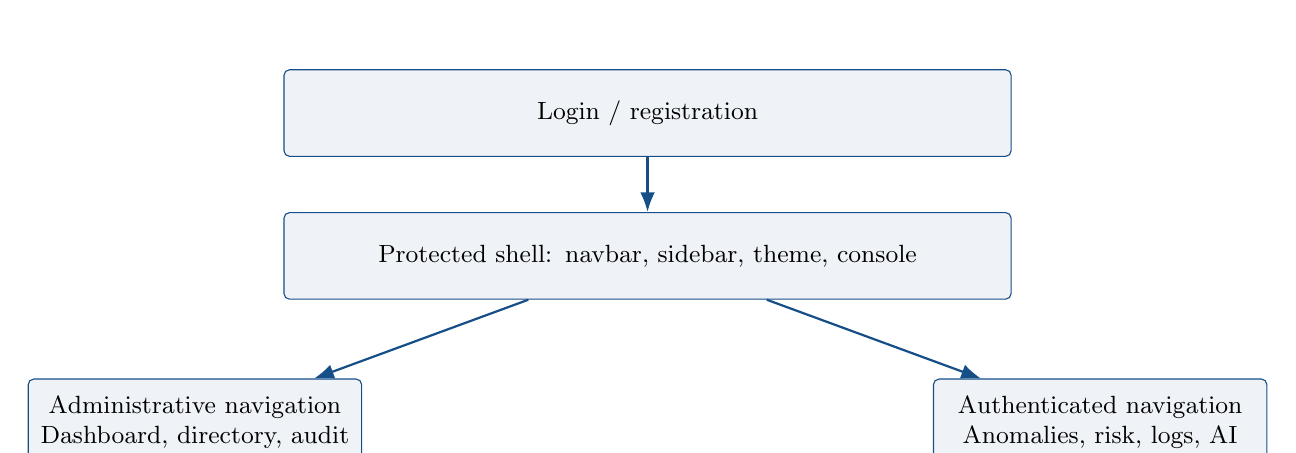
\begin{tikzpicture}[node distance=0.7cm]
\node[box,text width=9cm] (l) {Login / registration};
\node[box,below=of l,text width=9cm] (s) {Protected shell: navbar, sidebar, theme, console};
\node[box,below left=1cm and -1cm of s,text width=4cm] (a) {Administrative navigation\\Dashboard, directory, audit};
\node[box,below right=1cm and -1cm of s,text width=4cm] (u) {Authenticated navigation\\Anomalies, risk, logs, AI};
\draw[flow](l)--(s);\draw[flow](s)--(a);\draw[flow](s)--(u);
\end{tikzpicture}\caption{Source-derived navigation; backend authorization still applies.}\end{figure}

\section{Authentication and Navigation}
Login is outside the protected layout. Authentication context saves token and safe user data in browser local storage. The shared client sends bearer credentials and clears authentication state after relevant unauthorized responses. Registration creates an ordinary user.

Persistence survives a page refresh, but local storage can be accessed by scripts running within the page. Tests should cover token expiry, injected scripts, and malformed stored data. Frontend route guards assist navigation but cannot replace API authorization.

\section{Dashboard and Anomalies}
The dashboard route is administrator-only. Its combined metrics provide entry points to accounts or incidents requiring investigation. The anomalies API supports filtering, pagination, identifier lookup, and user-scoped views. Investigation should begin with stored rule type, description, and linked event metadata before considering generated explanations.

An anomaly alone does not prove an account was compromised. For example, a changed IP can reflect legitimate movement or network changes. The interface should support comparing related events and account context rather than implying that every rule match is an attack.

\section{Risk and Login Logs}
The risk view uses the score and its 24-hour horizon. A high score indicates accumulated rule weights; a low score may also reflect absent or expired telemetry. The logs page lists events and includes an administrative simulation form. The form creates a supplied telemetry record and invokes rules; it does not perform a real password attempt or network attack.

Synthetic records should be identified in demonstrations so they are not mistaken for genuine authentication evidence. Testing should compare the explicit ingestion path and real authentication recording because their timestamp and input sources differ.

\section{Directory, Audit, and Console}
The users page supports administrator account operations and active-state management. The audit page displays selected persisted security events. The Winston console component supplies browser diagnostics and API activity. Console output and database audit events have different purposes and should not be described as a complete forensic trail without coverage and integrity tests.

\section{AI Workspace}
The AI page selects investigator, containment operator, or collaborative behavior. It accepts prompt, context, queued steering, and follow-ups, then copies queue values into the request before submission. Returned steps show tool invocations and outcomes alongside final Markdown text and availability indicators.

Fallback output can still rely on real application tools. Absence of live inference does not automatically make every registry action a dry run. Validation must establish what the fallback planner selects and what permissions are enforced.

\clearpage\section{Application Screenshots}
Six captures were selected to show the entry point, overall monitoring, event investigation, personal account scope, and AI workspace. They are reproduced from candidate-provided screenshots without changing the displayed content. Counts and scores describe the captured demonstration state, not evaluation results.

\begin{figure}[!ht]\centering
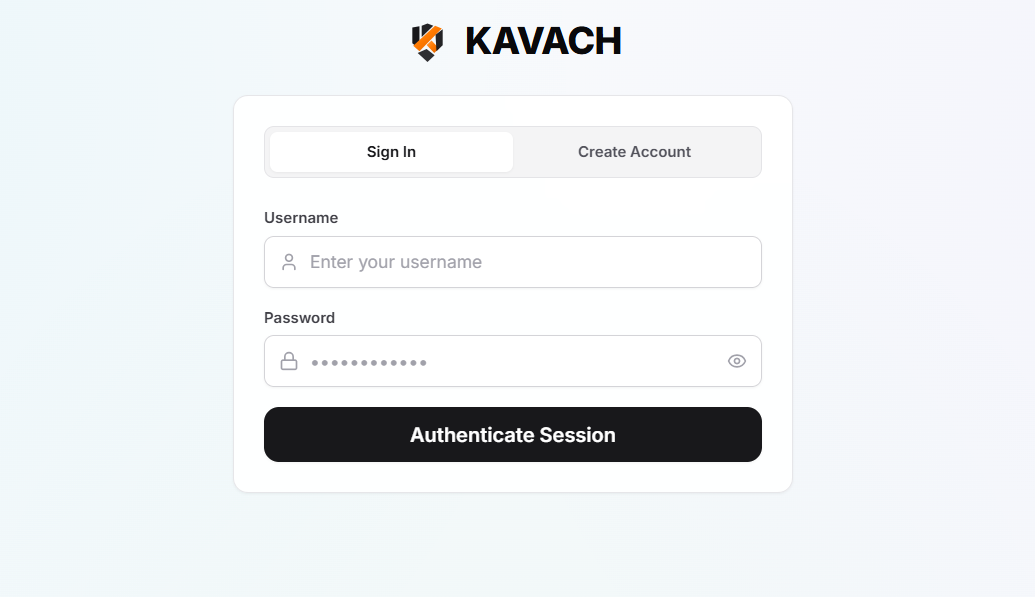
\includegraphics[width=.75\textwidth]{images/screenshot-login.png}
\caption{Sign-in interface with account-registration tab and authentication form.}\label{fig:screen-login}
\end{figure}

\begin{figure}[!ht]\centering
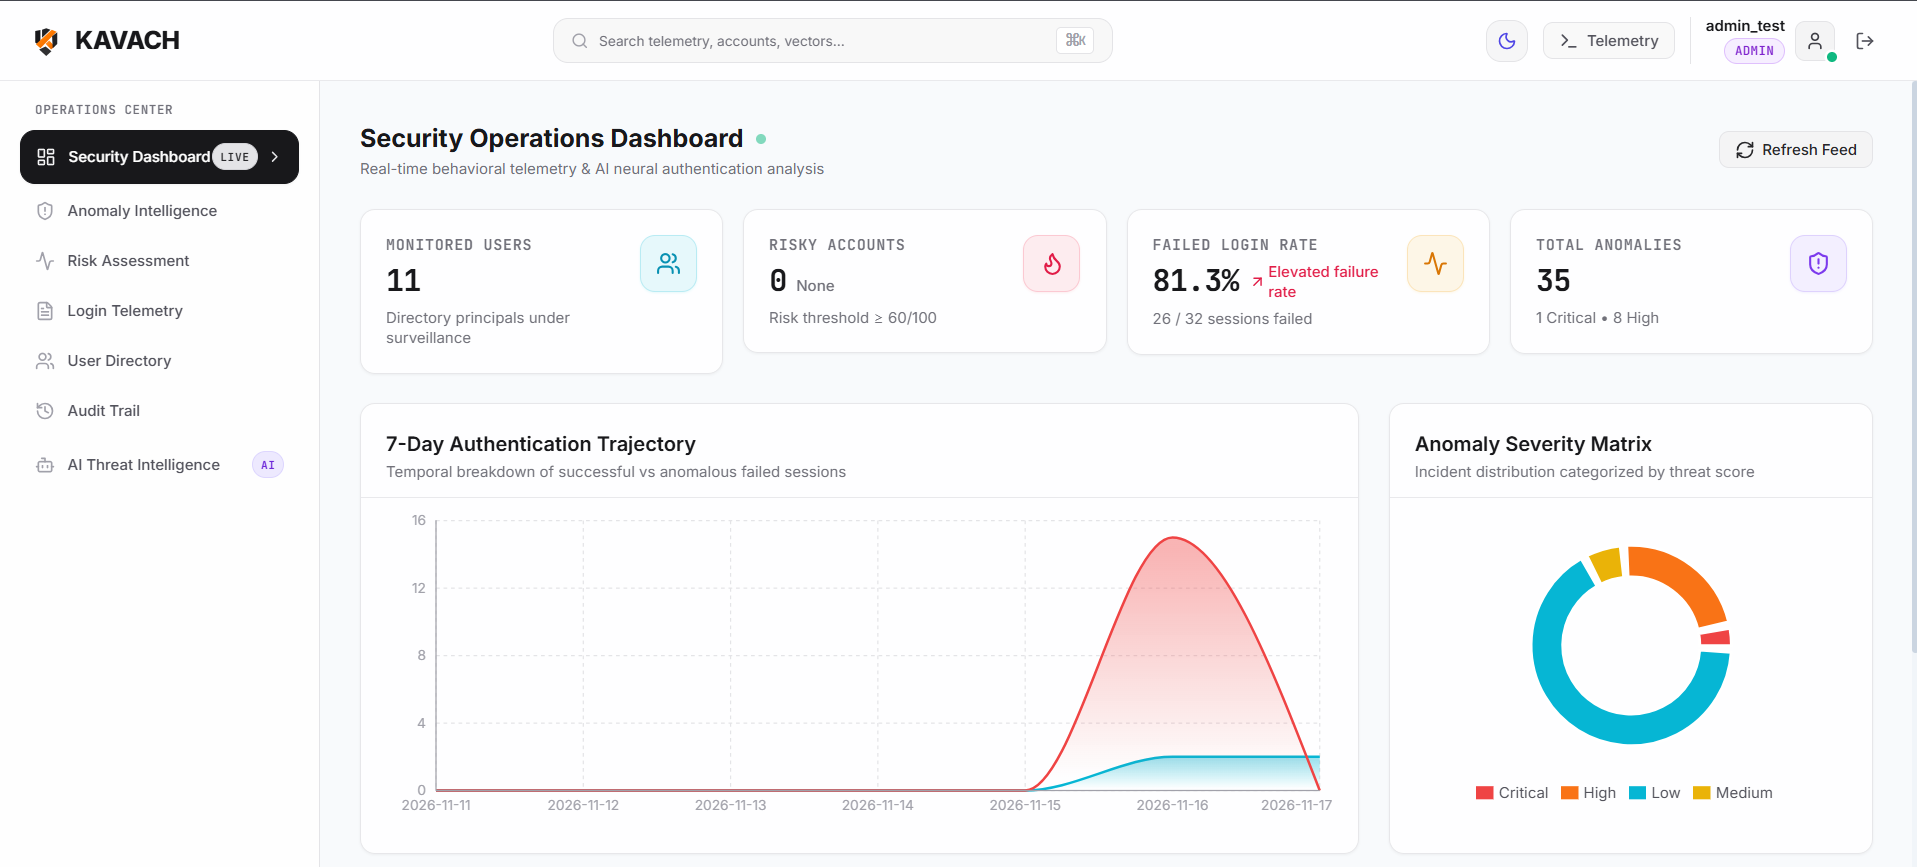
\includegraphics[width=\textwidth]{images/screenshot-dashboard.png}
\caption{Administrator dashboard: account counts, login outcomes, trend, and anomaly severity.}\label{fig:screen-dashboard}
\end{figure}

\clearpage\subsection{Anomaly Investigation and Login Telemetry}
The anomaly view exposes rule matches and per-alert weights, while the telemetry view shows the underlying login-event fields. Filters and action buttons are visible entry points; the captures do not show the outcomes of clicking those actions.

\begin{figure}[!ht]\centering
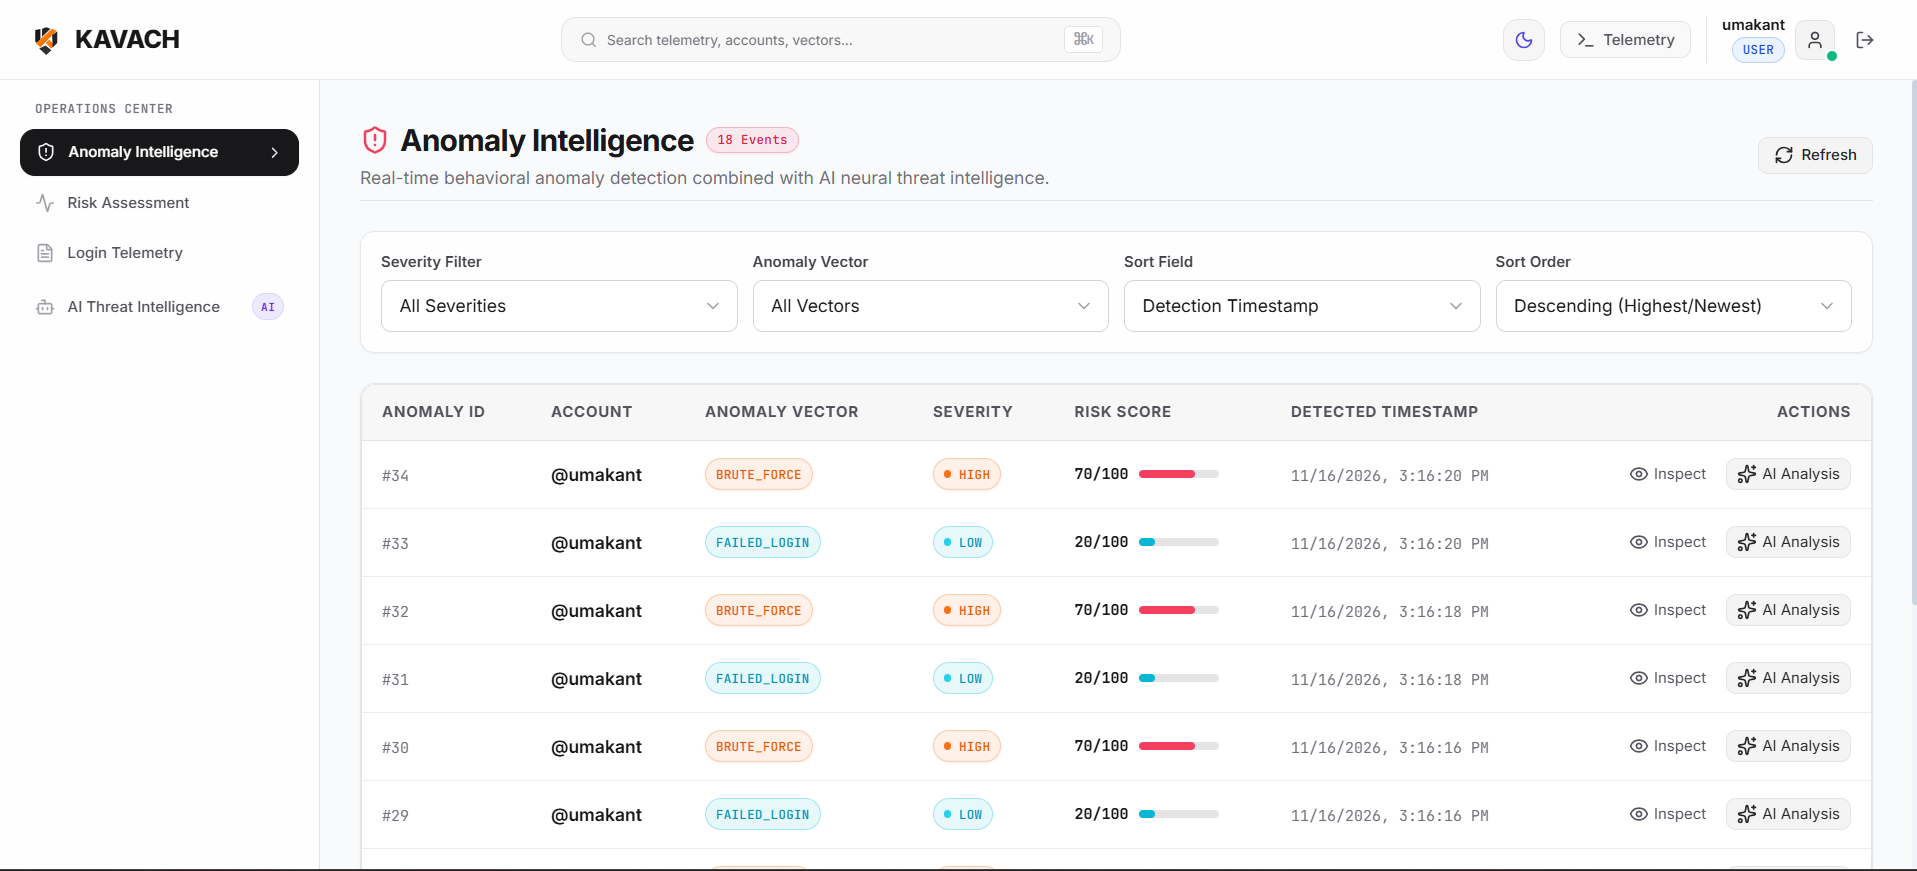
\includegraphics[width=\textwidth]{images/screenshot-anomalies.png}
\caption{User-scoped anomaly list with filters, rule types, severity, and alert weights.}\label{fig:screen-anomalies}
\end{figure}

\begin{figure}[!ht]\centering
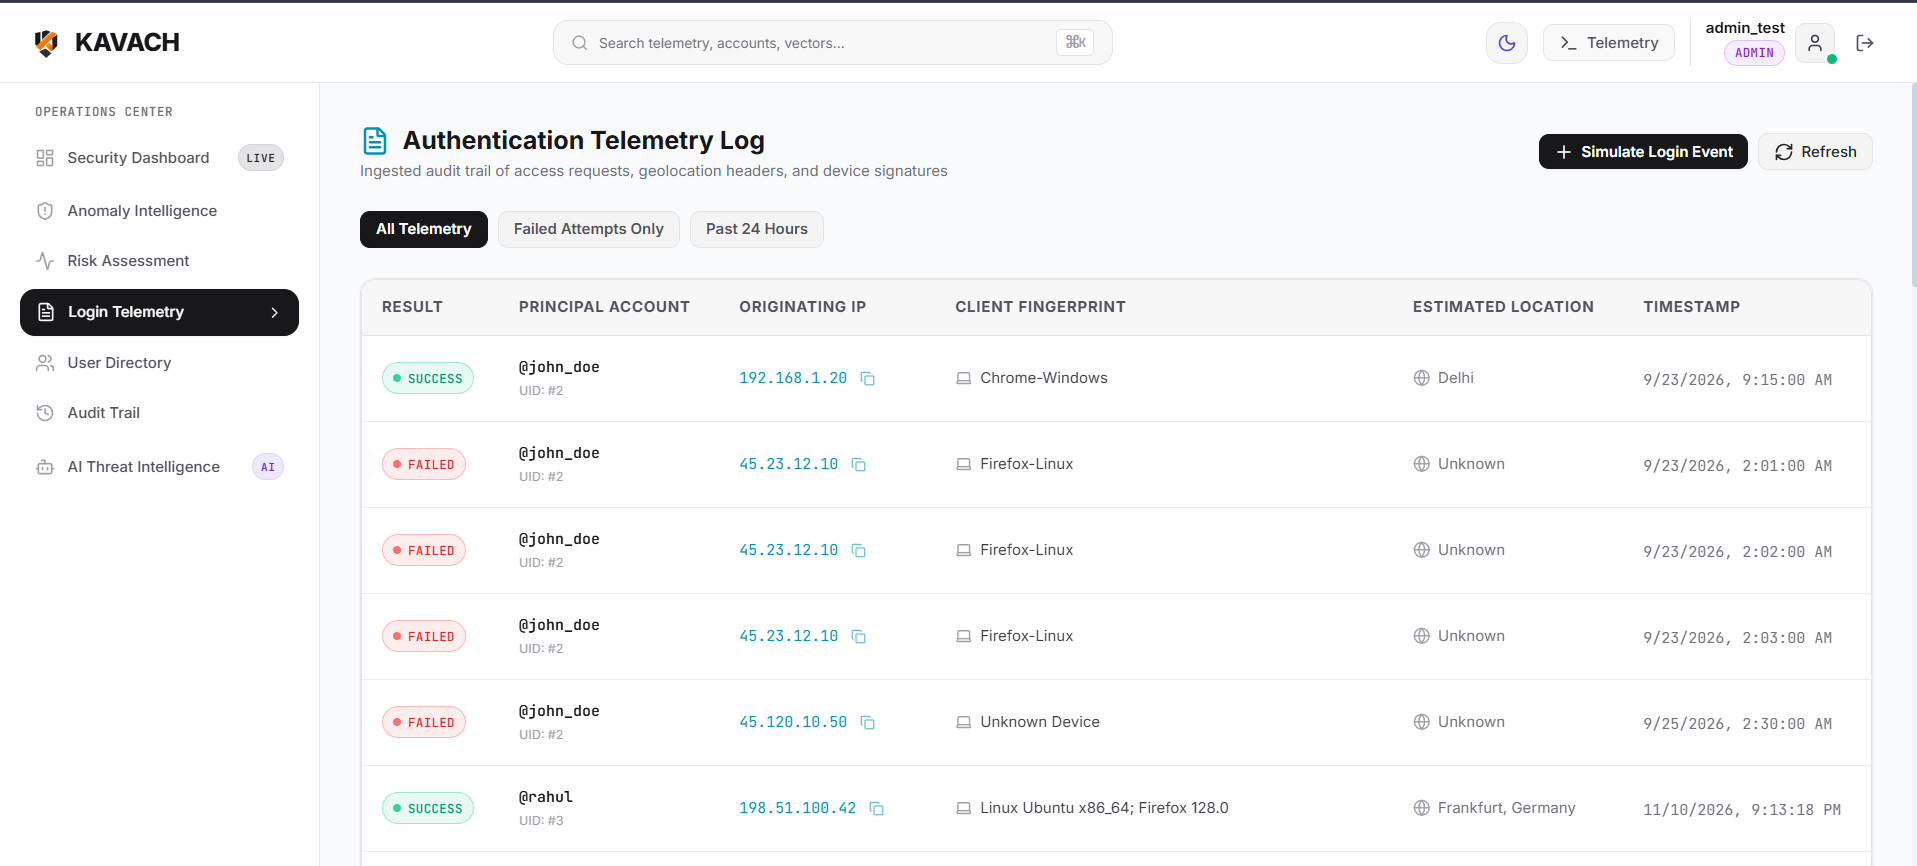
\includegraphics[width=\textwidth]{images/screenshot-telemetry.png}
\caption{Login telemetry showing successful and failed events with account and client metadata.}\label{fig:screen-telemetry}
\end{figure}

\clearpage\subsection{Personal Risk and AI Workspace}
The personal view displays the signed-in account's risk profile. Historical anomaly counts and the recent 24-hour risk score use different horizons. Interface subtitles such as ``Bayesian'' or ``neural'' do not alter the fixed-rule detector and additive score documented in Chapter 4. The AI capture shows its initial console state rather than a completed model or tool execution.

\begin{figure}[!ht]\centering
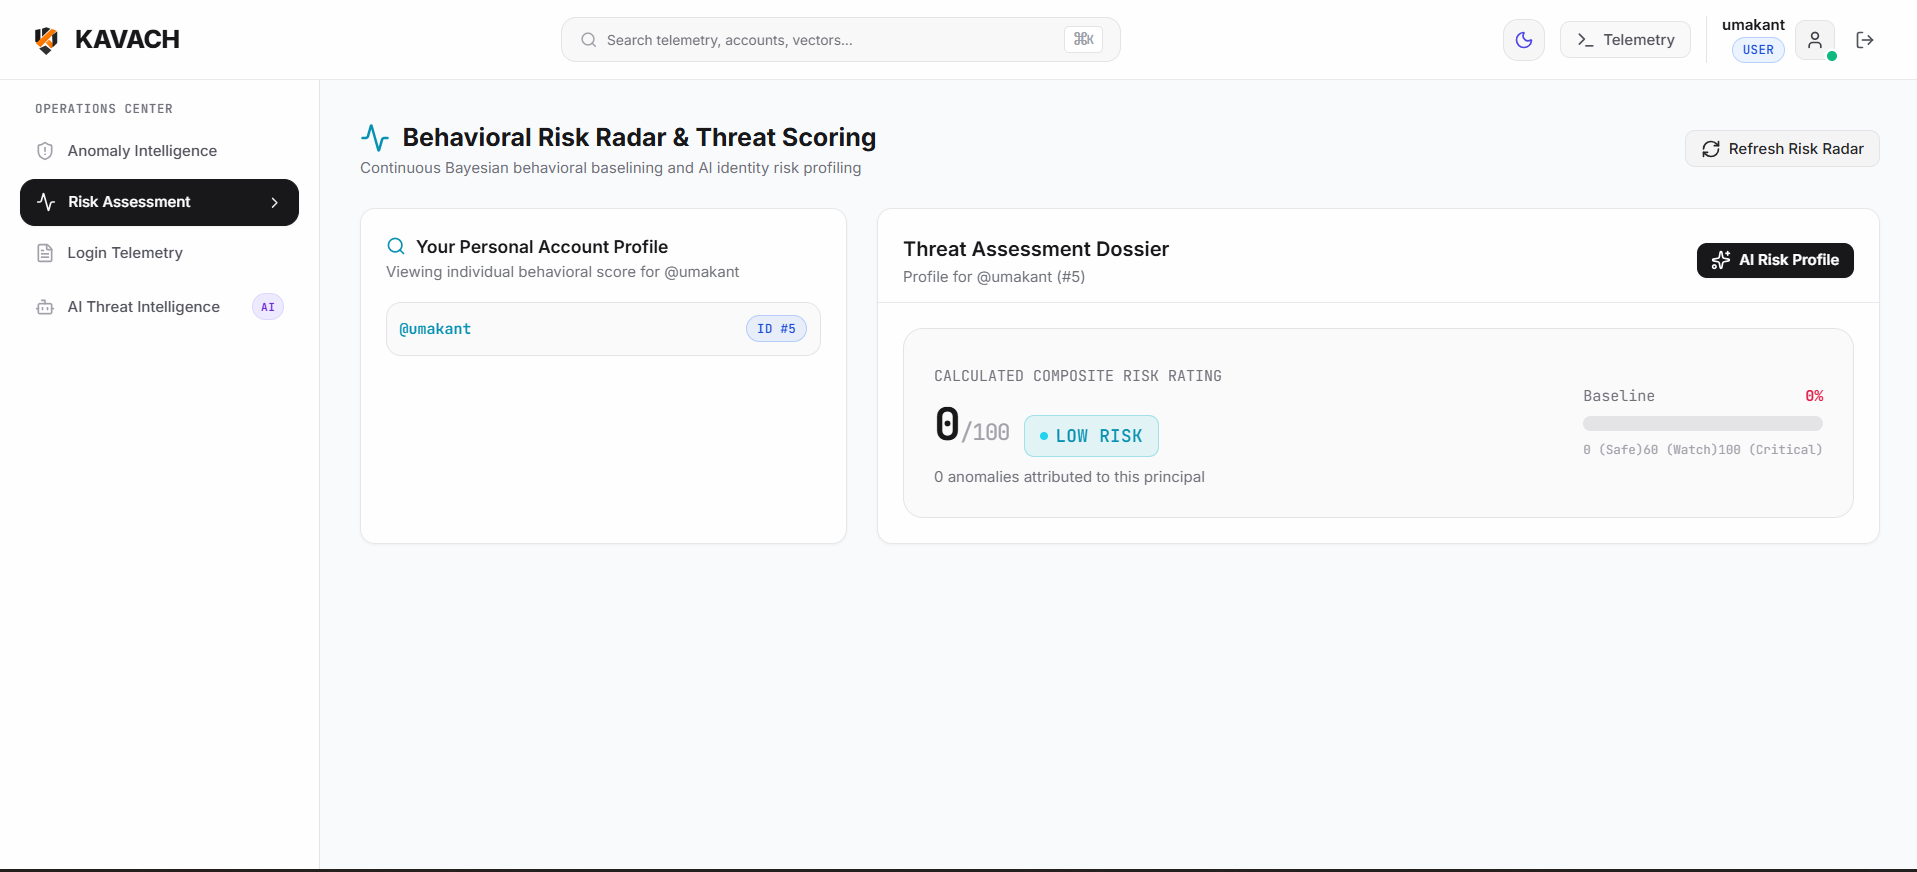
\includegraphics[width=\textwidth]{images/screenshot-personal-risk.png}
\caption{Personal risk view for the USER account, showing the displayed score and profile.}\label{fig:screen-risk}
\end{figure}

\begin{figure}[!ht]\centering
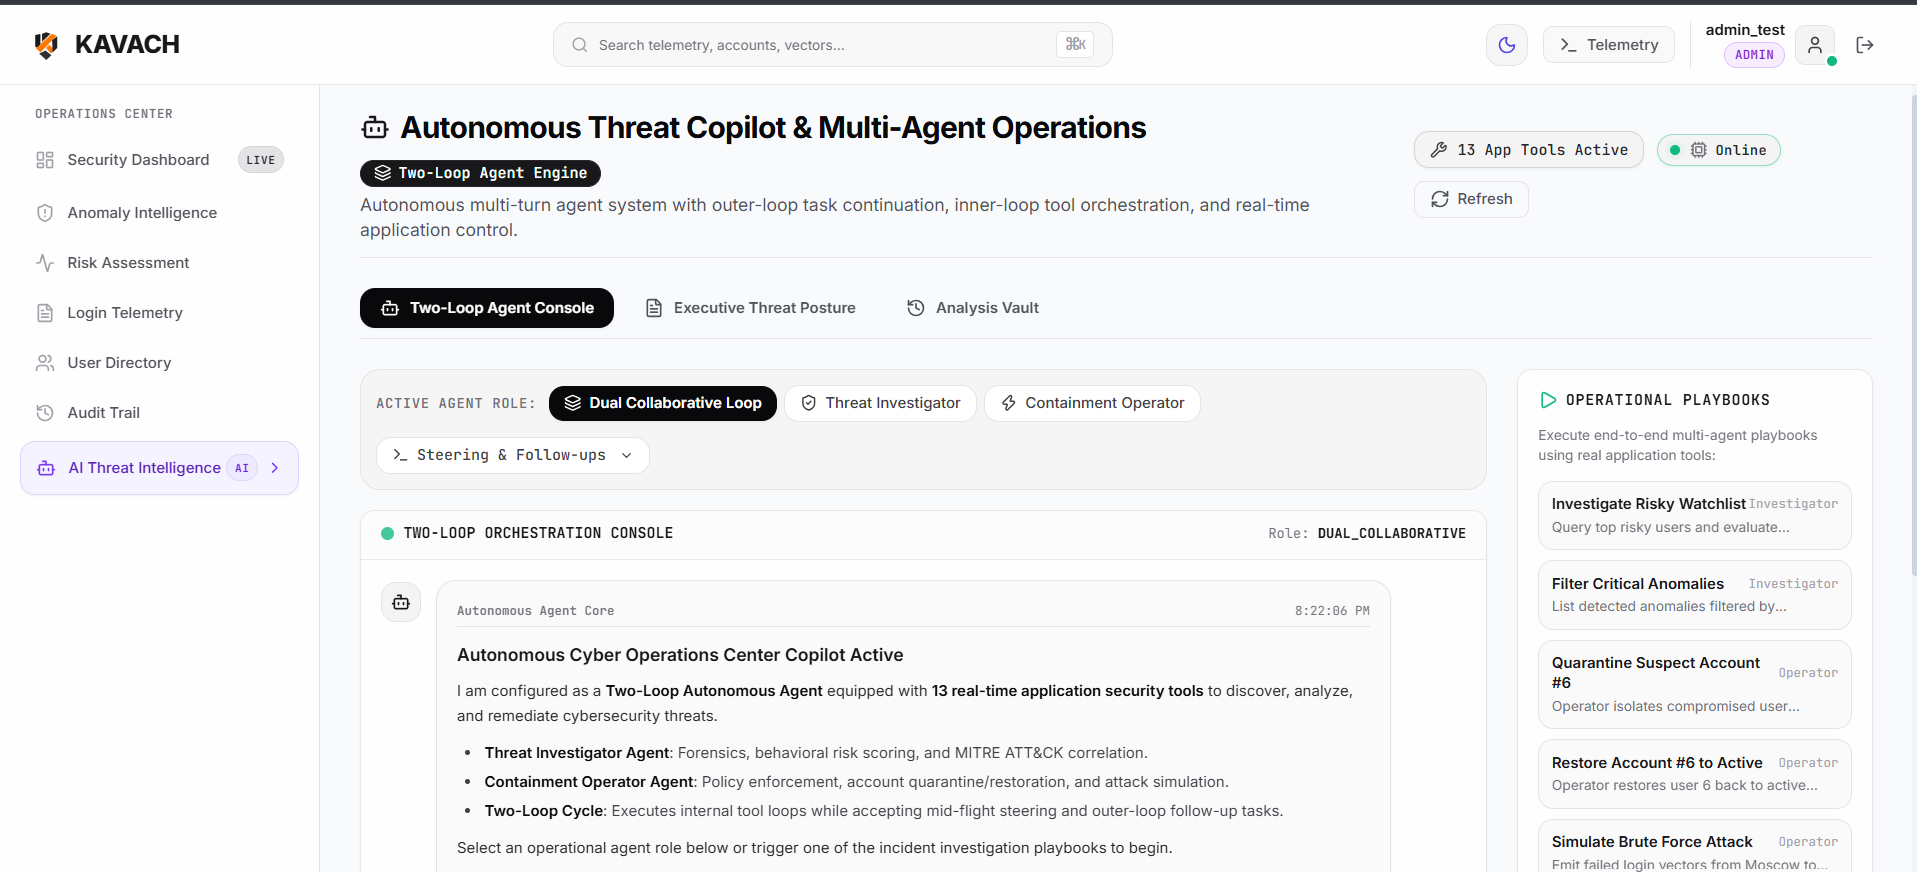
\includegraphics[width=\textwidth]{images/screenshot-ai-console.png}
\caption{AI workspace with agent-role selection, a 13-tool indicator, and operational playbooks.}\label{fig:screen-ai}
\end{figure}


\clearpage\section{Validation Status}
The repository contains one Spring Boot context-loading test. No rule-specific test-run results, labelled dataset, or load-test output was supplied. Source inspection and the candidate's screenshots support the implementation and interface descriptions. The screenshots are visual examples rather than a controlled execution of the validation plan. Table~\ref{tab:tests} lists proposed tests with expected behavior derived from the implementation; these are not recorded pass results.
\begingroup\small\setstretch{1.1}\setlength{\parskip}{0pt}
\begin{longtable}{>{\raggedright\arraybackslash}p{0.9cm}>{\raggedright\arraybackslash}p{6.1cm}>{\raggedright\arraybackslash}p{7cm}}
\caption{Functional validation plan; execution pending.}\label{tab:tests}\\\toprule ID & Input / action & Expected behavior to verify\\\midrule\endfirsthead
\toprule ID & Input / action & Expected behavior to verify\\\midrule\endhead
T1 & Register unique credentials. & Active USER, encoded password, safe response, audit event.\\
T2 & Repeat username or email. & Conflict and no duplicate account.\\
T3 & Valid password for active user. & JWT, success telemetry, applicable contextual rules.\\
T4 & Incorrect password for known user. & Unauthorized; failed telemetry and failed-login anomaly.\\
T5 & Unknown username. & Audit failure; no user-linked login record.\\
T6 & Inactive account attempts login. & Forbidden; failed telemetry and inactive-user anomaly.\\
T7 & Events at 04:59 and 05:00. & Unusual-time alert only before 05:00.\\
T8 & First event, repeated values, unseen IP/device. & No initial new-value alerts; later unseen values trigger.\\
T9 & Four then five failures in window. & Fifth qualifying failure adds brute-force anomaly.\\
T10 & Reanalyse identical login event. & No duplicate event/user/rule anomaly in sequential execution.\\
T11 & Weight totals 29, 30, 59, 60, 79, 80, 120. & Correct boundary tiers; score capped at 100.\\
T12 & Move anomaly detection time beyond 24 hours. & Expired anomaly excluded from risk.\\
T13 & Deactivate account with issued JWT. & Subsequent protected request rejected.\\
T14 & Make live inference unavailable. & Deterministic fallback with accurate status and outcomes.\\
T15 & Submit steering and two follow-ups. & Inner context consumes steering; outer cycles consume follow-ups.\\\bottomrule
\end{longtable}
\endgroup

\section{Security and Boundary Tests}
Test a USER requesting another account's logs, anomalies, and risk. Test directory changes through both direct REST and agent tools. Unauthorized data or actions should be denied. Tool-path tests matter because the inspected source uses differing call boundaries.

Exercise missing arguments, negative limits, oversized strings, invalid statuses, nonexistent IDs, and unknown tools. Feed malformed model JSON, provider errors, and misleading instructions inside tool results. Check failure during multi-step writes and concurrent anomaly insertion.

Time tests should include the exact ten-minute boundary, a backdated event with later failures already stored, and a recently inserted historical event. These distinguish strict ``after'' predicates, absent upper bounds, and login time from detection time.

\section{Empirical Evaluation Plan}
After functional validation, use a labelled corpus combining representative ordinary activity and controlled suspicious cases. Calculate precision and recall per rule and for the combined alert stream. Measure persistence, detection, dashboard queries, and model requests separately. Record hardware, database size, versions, concurrency, provider mode, and repeated runs.

Keep deterministic-fallback results separate from live-model results. Until measurements exist, the supported conclusion is that the source implements an inspectable monitoring workflow, with empirical effectiveness still to be established.
\chapter{Conclusion and Future Work}
\section{Conclusion}
KAVACH integrates authentication telemetry, six deterministic rules, recent user risk, dashboard summaries, audit records, and a tool-assisted AI workflow. Frontend pages, API controllers, services, repositories, and entities make the processing stages traceable.

The detector provides explicit reasons and fixed weights. The risk service summarizes recent evidence in a bounded score. Structured explanations and the two-loop interface add an investigation mechanism with deterministic fallback. Together, these components support a practical application-level security-monitoring demonstration.

The evidence supports implementation conclusions, not production-readiness claims, detection accuracy, or measured latency improvements. This report identifies the tests required to assess those properties instead of assigning unsupported figures.

\section{Current Limitations}
The fixed off-hours rule does not learn personal schedules. IP/device baselines use strings, can include failures, and do not establish hardware identity or geographic plausibility. Weights lack empirical calibration, and multiple alerts from a single event can saturate risk quickly.

The brute-force query has no explicit event-time upper bound. Time conventions and historical input need careful handling. Some queries read full history, and duplicate prevention requires concurrency validation. Agent tools combine queries and state changes, making consistent authorization essential. Steering is request-local, execution is sequential, and the frontend timeout may be shorter than a multi-cycle agent request.

\section{Future Direction of Work}
\subsection{Centralized Tool Policy}
Check authenticated principal, action, resource ownership, and arguments before every tool invocation. Introduce review or approval for consequential changes where appropriate. Record the initiating principal, target, outcome, and rationale instead of relying only on generated narrative.

\subsection{Detection and Data Quality}
Adopt a consistent time-zone-aware timestamp convention, enforce intended event windows, and test out-of-order input. Consider successful-login baselines and bounded history for IP/device rules. Calibrate thresholds using representative labelled data and publish false positives as well as detections.

\subsection{Audit Integrity and Reliability}
Add appropriate uniqueness constraints, transaction tests, and telemetry-failure monitoring. Define retention and access controls. If stronger integrity is needed, evaluate append-only storage, external export, or tamper-evident verification instead of assuming database persistence supplies it.

\subsection{Agent Sessions and Interaction}
Introduce authenticated job/session identifiers and a channel for progress, steering, and cancellation. Bound outer-loop work and request size; make operational tools idempotent where possible. Report the actual inference/fallback mode used for each result and align client timeouts with server execution.

\subsection{Scale and Evaluation}
Replace growing history scans with bounded queries, review indexes with query plans, and measure concurrent load. Build integration tests and a labelled evaluation corpus before adding learned anomaly models or external SIEM ingestion. Additional authentication factors and stronger browser token handling are further deployment options.

\section{Closing Perspective}
The project's principal contribution is the integration of transparent detection and recent risk with an inspectable investigation interface. Completing validation and enforcing policy at the tool boundary would provide a firmer basis for evaluating use beyond a development demonstration.

\begin{thebibliography}{9}
\bibitem{repo} KAVACH project source, \emph{login-analysis-backend} and \emph{login-analysis-frontend}, local snapshot reviewed 17 November 2026. Source map in Appendix A.
\bibitem{jwt} M. Jones, J. Bradley, and N. Sakimura, \emph{JSON Web Token (JWT)}, RFC 7519, May 2015. \url{https://www.rfc-editor.org/rfc/rfc7519}.
\bibitem{spring} Spring, \emph{Spring Security Reference: Method Security}. \url{https://docs.spring.io/spring-security/reference/servlet/authorization/method-security.html}. Accessed 17 November 2026.
\bibitem{owasp} OWASP Foundation, \emph{Logging Cheat Sheet}. \url{https://cheatsheetseries.owasp.org/cheatsheets/Logging_Cheat_Sheet.html}. Accessed 17 November 2026.
\bibitem{template} NIT Agartala, \emph{B.Tech 7th Semester LaTeX Template}, user-supplied archive including institutional class, logos, and chapter styling; adapted for MCA.
\end{thebibliography}
\appendix% Supporting material after References.
\chapter{Project Structure}
\section{Repository Organization}
KAVACH separates its REST backend from its browser frontend. The following tree shows the application directories relevant to the implementation. Generated build output, dependency folders, and local configuration values are omitted.
\begingroup\footnotesize\setstretch{1.0}
\begin{lstlisting}[basicstyle=\ttfamily\scriptsize]
UserLoginProject/
  login-analysis-backend/
    pom.xml, mvnw, mvnw.cmd
    src/main/java/com/loginanalysis/
      LoginAnalysisBackendApplication.java
      config/       JWT filter, security, passwords, AI setup
      controller/   REST entry points
      dto/          Request and response contracts
      entity/       JPA model
      repository/   Queries and aggregates
      service/      Business logic
      agent/
        TwoLoopAgentService.java
        model/      Roles, messages, tools, execution steps
        tools/      SecurityToolsRegistry.java
      util/         Provider and request helpers
      exception/    Application errors
    src/main/resources/application.properties
    src/test/java/com/loginanalysis/
      LoginAnalysisBackendApplicationTests.java
  login-analysis-frontend/
    package.json, vite.config.js
    public/
    src/
      App.jsx, main.jsx
      api/          HTTP client and feature APIs
      context/      Authentication and theme
      pages/        Feature pages
      components/   Layout and reusable UI
      utils/        Logging and animation
      assets/
\end{lstlisting}
\endgroup

\clearpage\section{Principal Implementation Modules}
Table~\ref{tab:appendix-modules} lists implementation responsibilities. The backend package root is shown below; frontend paths start at \code{login-analysis-frontend/src/}.
\par{\footnotesize\code{login-analysis-backend/src/main/java/com/loginanalysis/}}\par
\begingroup\footnotesize\setstretch{1.0}\setlength{\parskip}{0pt}\renewcommand{\arraystretch}{1.1}
\begin{longtable}{>{\raggedright\arraybackslash}p{3.8cm}>{\raggedright\arraybackslash}p{10.3cm}}
\caption{Principal application modules and responsibilities.}\label{tab:appendix-modules}\\\toprule Responsibility & Modules\\\midrule\endfirsthead
\toprule Responsibility & Modules\\\midrule\endhead
Authentication & \code{service/AuthService.java}, \code{service/JwtService.java}, \code{config/PasswordConfig.java}.\\
Access control & \code{config/SecurityConfig.java}, \code{config/JwtAuthenticationFilter.java}, \code{service/UserAuthorizationService.java}.\\
Telemetry and detection & \code{service/LoginLogService.java}, \code{service/AnomalyDetectionService.java}, \code{repository/LoginLogRepository.java}.\\
Risk and analytics & \code{service/RiskService.java}, \code{service/LoginAnalyticsService.java}, \code{service/SecurityDashboardService.java}, \code{repository/AnomalyRepository.java}.\\
User and audit operations & \code{service/UserService.java}, \code{service/AuditLogService.java}, and their controllers/repositories.\\
AI explanations & \code{service/GrokAIService.java}, \code{util/GrokClient.java}, \code{config/GrokConfig.java}.\\
Agent execution & \code{agent/TwoLoopAgentService.java}, \code{agent/tools/SecurityToolsRegistry.java}, \code{agent/model/AgentTool.java}.\\
API contracts & \code{controller/AIAnalysisController.java} and the request/response classes in \code{dto/}.\\
Frontend state and routing & \code{App.jsx}, \code{context/AuthContext.jsx}, \code{context/ThemeContext.jsx}, \code{api/client.js}.\\
Frontend views & \code{pages/LoginPage.jsx}, \code{DashboardPage.jsx}, \code{AnomaliesPage.jsx}, \code{RiskPage.jsx}, \code{LoginLogsPage.jsx}, \code{UsersPage.jsx}, \code{AuditPage.jsx}, and \code{GrokAiPage.jsx} within \code{pages/}.\\\bottomrule
\end{longtable}\endgroup

The backend follows a controller--service--repository organization. Request DTOs define inputs, services coordinate business operations, and repositories query mapped entities. The frontend uses a shared Axios client and common authentication state. The agent registry is an additional service entry path; it must be considered alongside direct controller calls when assessing authorization.

\chapter{Database Tables}
The dictionary documents JPA attributes and Java types, with explicit column names where declared. PK means primary key, FK relationship, NN non-null, and UQ unique. All IDs use identity-generated Long values; enums are stored as strings. Initialization values describe application defaults, not SQL DEFAULT clauses. Physical naming follows ORM configuration.

\section{Users}
\begingroup\footnotesize\setstretch{1.0}\setlength{\parskip}{0pt}\renewcommand{\arraystretch}{1.15}
\begin{longtable}{>{\raggedright\arraybackslash}p{4.5cm}>{\raggedright\arraybackslash}p{2.2cm}>{\raggedright\arraybackslash}p{1.4cm}>{\raggedright\arraybackslash}p{5.7cm}}
\caption{Data dictionary: \code{users}.}\\\toprule Attribute & Type & Mapping & Purpose / initialization\\\midrule\endfirsthead
\toprule Attribute & Type & Mapping & Purpose / initialization\\\midrule\endhead
\code{id} & Long & PK & Identity-generated account identifier.\\
\code{username} & String & NN, UQ & Up to 100 characters.\\
\code{email} & String & NN, UQ & Up to 150 characters; normalized during registration.\\
\code{password} & String & NN & Encoded password; authentication uses BCrypt matching.\\
\code{active} & Boolean & NN & Initialized to true; false blocks account access.\\
\code{role} & UserRole & NN & String enum, length 20; initialized to USER when absent.\\
\code{createdAt} & LocalDate\allowbreak{}Time & NN & Set on creation when absent.\\\bottomrule
\end{longtable}\endgroup

\noindent\textbf{Relationships:} one user can have many login records, anomalies, and analysis-history records. The audit entity stores a username string and does not declare a relationship to \code{users}. UserRole values are ADMIN and USER.

\section{Login Events}
\begingroup\footnotesize\setstretch{1.0}\setlength{\parskip}{0pt}\renewcommand{\arraystretch}{1.15}
\begin{longtable}{>{\raggedright\arraybackslash}p{4.5cm}>{\raggedright\arraybackslash}p{2.2cm}>{\raggedright\arraybackslash}p{1.4cm}>{\raggedright\arraybackslash}p{5.7cm}}
\caption{Data dictionary: \code{user_login_logs}.}\\\toprule Attribute / column & Type & Mapping & Purpose\\\midrule\endfirsthead
\toprule Attribute / column & Type & Mapping & Purpose\\\midrule\endhead
\code{id} & Long & PK & Login-event identifier.\\
\code{user} / \code{user_id} & User & FK, NN & Required many-to-one, lazy user reference.\\
\code{loginTime} / \code{login_time} & LocalDate\allowbreak{}Time & NN & Event timestamp; initialized when absent.\\
\code{ipAddress} / \code{ip_address} & String & NN & Up to 100 characters.\\
\code{location} & String & Optional & Up to 100 characters; event-supplied context.\\
\code{device} & String & Optional & Up to 200 characters; device/user-agent string.\\
\code{status} & LoginStatus & NN & String enum, length 20: SUCCESS or FAILED.\\\bottomrule
\end{longtable}\endgroup
Indexes are declared on \code{user_id}, \code{login_time}, \code{status}, and \code{ip_address}. Their entity names are \code{idx_login_username}, \code{idx_login_time}, \code{idx_login_status}, and \code{idx_login_ip}, respectively. Despite its name, \code{idx_login_username} indexes the user identifier.

\section{Anomalies}
\begingroup\footnotesize\setstretch{1.0}\setlength{\parskip}{0pt}\renewcommand{\arraystretch}{1.15}
\begin{longtable}{>{\raggedright\arraybackslash}p{4.5cm}>{\raggedright\arraybackslash}p{2.2cm}>{\raggedright\arraybackslash}p{1.4cm}>{\raggedright\arraybackslash}p{5.7cm}}
\caption{Data dictionary: \code{anomalies}.}\\\toprule Attribute / column & Type & Mapping & Purpose\\\midrule\endfirsthead
\toprule Attribute / column & Type & Mapping & Purpose\\\midrule\endhead
\code{id} & Long & PK & Anomaly identifier.\\
\code{user} / \code{user_id} & User & FK, NN & Required many-to-one account reference.\\
\code{loginLog} / \code{login_log_id} & LoginLog & FK, NN & Required triggering-event reference.\\
\code{anomalyType} & AnomalyType & NN & One of the six rule types.\\
\code{description} & String & NN & Human-readable trigger explanation.\\
\code{riskScore} & Integer & NN & Fixed weight assigned by the matching rule.\\
\code{severity} & Severity & NN & LOW, MEDIUM, HIGH, or CRITICAL.\\
\code{detectedAt} & LocalDate\allowbreak{}Time & NN & Detection timestamp initialized when saved.\\\bottomrule
\end{longtable}\endgroup

The six types are \code{FAILED_LOGIN}, \code{UNUSUAL_LOGIN_TIME}, \code{INACTIVE_USER_LOGIN}, \code{NEW_IP}, \code{NEW_DEVICE}, and \code{BRUTE_FORCE}. The service checks for an existing user/type/login combination before insertion; the entity does not declare a corresponding composite uniqueness constraint.

\section{AI Analysis History}
\begingroup\footnotesize\setstretch{1.0}\setlength{\parskip}{0pt}\renewcommand{\arraystretch}{1.15}
\begin{longtable}{>{\raggedright\arraybackslash}p{4.5cm}>{\raggedright\arraybackslash}p{2.2cm}>{\raggedright\arraybackslash}p{1.4cm}>{\raggedright\arraybackslash}p{5.7cm}}
\caption{Data dictionary: \code{ai_analysis_history}.}\\\toprule Attribute / column & Type & Mapping & Purpose\\\midrule\endfirsthead
\toprule Attribute / column & Type & Mapping & Purpose\\\midrule\endhead
\code{id} & Long & PK & Analysis record identifier.\\
\code{anomaly} / \code{anomaly_id} & Anomaly & FK, optional & Lazy link to the analyzed anomaly.\\
\code{user} / \code{user_id} & User & FK, optional & Lazy link to the associated user.\\
\code{cachedAnomalyId} & Long & Optional & Column \code{cached_anomaly_id}; retained identifier, not FK.\\
\code{cachedUserId} & Long & Optional & Column \code{cached_user_id}; retained identifier, not FK.\\
\code{username} & String & Optional & Up to 100 characters.\\
\code{analysisType} & String & NN & Up to 50 characters.\\
\code{summary} & String / TEXT & Optional & Generated or fallback overview.\\
\code{riskExplanation} & String / TEXT & Optional & Contextual risk explanation.\\
\code{indicatorsJson} & String / TEXT & Optional & Serialized indicators.\\
\code{recommendationsJson} & String / TEXT & Optional & Serialized recommendations.\\
\code{confidence} & String & Optional & Up to 20 characters; advisory label.\\
\code{threatLevel} & String & Optional & Up to 20 characters.\\
\code{model} & String & Optional & Up to 100 characters.\\
\code{isAdvisory} & Boolean & NN & Initialized to true.\\
\code{createdAt} & LocalDate\allowbreak{}Time & NN & Analysis creation timestamp.\\\bottomrule
\end{longtable}\endgroup

The JSON-labelled fields are mapped as TEXT, not as PostgreSQL JSONB in these entity definitions. Optional links and cached identifiers retain contextual information; the history DTO and service determine what is returned to the caller.

\section{Audit Records}
\begingroup\footnotesize\setstretch{1.0}\setlength{\parskip}{0pt}\renewcommand{\arraystretch}{1.15}
\begin{longtable}{>{\raggedright\arraybackslash}p{4.5cm}>{\raggedright\arraybackslash}p{2.2cm}>{\raggedright\arraybackslash}p{1.4cm}>{\raggedright\arraybackslash}p{5.7cm}}
\caption{Data dictionary: \code{audit_logs}.}\\\toprule Attribute & Type & Mapping & Purpose\\\midrule\endfirsthead
\toprule Attribute & Type & Mapping & Purpose\\\midrule\endhead
\code{id} & Long & PK & Audit record identifier.\\
\code{username} & String & Optional & Actor/account text; no declared user FK.\\
\code{action} & String & NN & Security or application action name.\\
\code{details} & String & Optional & Description, up to 1000 characters.\\
\code{ipAddress} & String & Optional & Recorded request/action source.\\
\code{timestamp} & LocalDate\allowbreak{}Time & NN & Initialized when absent.\\\bottomrule
\end{longtable}\endgroup
The audit table persists selected events. The entity does not establish append-only enforcement, hash chaining, or a database-trigger-based complete change log.

\chapter{API Quick Reference}
All routes start with \code{/api}; \code{:name} denotes a path variable. Public requires no token. ADMIN/USER are application roles; Owner permits an administrator or the checked account owner. Signed-in denotes the general authentication requirement. Scopes document source declarations, not executed authorization tests; agent tools require separate execution policy.

\section{Authentication and Directory}
\begingroup\footnotesize\setstretch{1.0}\setlength{\parskip}{0pt}\renewcommand{\arraystretch}{1.15}
\begin{longtable}{>{\raggedright\arraybackslash}p{1.5cm}>{\raggedright\arraybackslash}p{5.9cm}>{\raggedright\arraybackslash}p{1.8cm}>{\raggedright\arraybackslash}p{4.6cm}}
\caption{Authentication and user-directory endpoints.}\\\toprule Method & Route after /api & Scope & Purpose\\\midrule\endfirsthead
\toprule Method & Route after /api & Scope & Purpose\\\midrule\endhead
POST & \code{/auth/register} & Public & Register an active USER; returns 201 and safe account details.\\
POST & \code{/auth/login} & Public & Verify credentials; return JWT and safe account details.\\
GET & \code{/users} & ADMIN & List accounts.\\
POST & \code{/users} & ADMIN & Create an account; returns 201.\\
GET & \code{/users/:id} & ADMIN & Retrieve an account.\\
PUT & \code{/users/:id} & ADMIN & Update account using UserRequestDTO.\\
PATCH & \code{/users/:id/status?active=false} & ADMIN & Set active state; query parameter can be true or false.\\
DELETE & \code{/users/:id} & ADMIN & Delete account; returns 204 on completion.\\\bottomrule
\end{longtable}\endgroup

Registration requires \code{username}, \code{email}, and \code{password}. The DTO limits username to 3--100 characters, email to 150, and password to 8--72. Login requires nonblank username/password and limits them to 100/72 characters. A failed known-account login attempts telemetry recording; an unknown account produces an audit failure without user-linked telemetry.

\section{Telemetry and Anomalies}
\begingroup\footnotesize\setstretch{1.0}\setlength{\parskip}{0pt}\renewcommand{\arraystretch}{1.15}
\begin{longtable}{>{\raggedright\arraybackslash}p{1.5cm}>{\raggedright\arraybackslash}p{5.9cm}>{\raggedright\arraybackslash}p{1.8cm}>{\raggedright\arraybackslash}p{4.6cm}}
\caption{Login-event and anomaly endpoints.}\\\toprule Method & Route after /api & Scope & Purpose\\\midrule\endfirsthead
\toprule Method & Route after /api & Scope & Purpose\\\midrule\endhead
POST & \code{/login-logs} & ADMIN & Persist an explicit event and invoke detection.\\
GET & \code{/login-logs} & ADMIN & List login records.\\
GET & \code{/login-logs/user/:userId} & Owner & Retrieve account-specific logs.\\
GET & \code{/login-logs/failed} & ADMIN & Retrieve failed events.\\
GET & \code{/login-logs/recent?hours=24} & ADMIN & Retrieve recent events; hours defaults to 24.\\
GET & \code{/anomalies} & ADMIN & Paginated list with severity/type filters and sorting.\\
GET & \code{/anomalies/:id} & Owner & Retrieve one anomaly; check its owning account.\\
GET & \code{/anomalies/user/:userId} & Owner & List an account's anomalies.\\
GET & \code{/anomalies/user/:userId/paginated} & Owner & Paginated account anomalies and filters.\\
GET & \code{/anomalies/severity/:severity} & ADMIN & List anomalies by severity.\\
GET & \code{/anomalies/type/:type} & ADMIN & List anomalies by rule type.\\\bottomrule
\end{longtable}\endgroup

Explicit event input requires \code{userId}, \code{ipAddress}, and \code{status}; \code{loginTime}, \code{location}, and \code{device} are optional. Anomaly pagination defaults to \code{page=0}, \code{size=10}, \code{sortBy=detectedAt}, and \code{direction=desc}. Page must be nonnegative, size must be 1--100, and allowed sort fields are \code{id}, \code{detectedAt}, \code{riskScore}, \code{severity}, and \code{anomalyType}.

\section{Risk, Dashboard, and Audit}
\begingroup\footnotesize\setstretch{1.0}\setlength{\parskip}{0pt}\renewcommand{\arraystretch}{1.15}
\begin{longtable}{>{\raggedright\arraybackslash}p{1.5cm}>{\raggedright\arraybackslash}p{5.9cm}>{\raggedright\arraybackslash}p{1.8cm}>{\raggedright\arraybackslash}p{4.6cm}}
\caption{Risk, analytics, dashboard, and audit endpoints.}\\\toprule Method & Route after /api & Scope & Purpose\\\midrule\endfirsthead
\toprule Method & Route after /api & Scope & Purpose\\\midrule\endhead
GET & \code{/risk/user/:userId} & Owner & Account's 24-hour capped risk score and tier.\\
GET & \code{/risk/dashboard} & ADMIN & Overall risk/severity summary.\\
GET & \code{/dashboard/security} & ADMIN & Combined security dashboard.\\
GET & \code{/dashboard/top-risky-users} & ADMIN & Ranked watchlist, up to ten accounts.\\
GET & \code{/dashboard/recent-critical-anomalies} & ADMIN & Recent critical anomalies.\\
GET & \code{/analytics/logins} & Signed-in & Login counts, failure rate, seven-day trend.\\
GET & \code{/audit-logs} & ADMIN & All persisted audit records.\\
GET & \code{/audit-logs/user/:username} & ADMIN & Audit records for a username.\\
GET & \code{/audit-logs/action/:action} & ADMIN & Audit records for an action.\\\bottomrule
\end{longtable}\endgroup

The analytics controller does not declare an ADMIN-only annotation on its login-analytics route; it inherits the authenticated-request requirement from the security chain. API consumers must distinguish this declaration from the administrator-only dashboard routes.

\section{AI Analysis and Agent Execution}
\begingroup\footnotesize\setstretch{1.0}\setlength{\parskip}{0pt}\renewcommand{\arraystretch}{1.15}
\begin{longtable}{>{\raggedright\arraybackslash}p{1.5cm}>{\raggedright\arraybackslash}p{5.9cm}>{\raggedright\arraybackslash}p{1.8cm}>{\raggedright\arraybackslash}p{4.6cm}}
\caption{AI and two-loop agent endpoints.}\\\toprule Method & Route after /api & Scope & Purpose\\\midrule\endfirsthead
\toprule Method & Route after /api & Scope & Purpose\\\midrule\endhead
GET & \code{/ai/status} & ADMIN / USER & Model readiness and mode information.\\
POST & \code{/ai/analyze/anomaly/:anomalyId} & Owner & Dedicated anomaly explanation; alias below.\\
POST & \code{/ai/analyze-anomaly/:anomalyId} & Owner & Alias for anomaly explanation.\\
GET / POST & \code{/ai/analyze/security-summary} & ADMIN & Global security summary; also \code{/ai/summary}.\\
GET & \code{/ai/history} & ADMIN / USER & Paginated history; service scopes ordinary users to their own records.\\
GET & \code{/ai/history/:id} & ADMIN / USER & One history record; service checks cached owner where present.\\
POST & \code{/ai/analyze-user/:userId} & Owner & Dedicated user-risk analysis.\\
POST & \code{/ai/agent-loop} & ADMIN / USER & Execute prompt and queued steering/follow-ups; return trace.\\
GET & \code{/ai/agent-tools} & ADMIN / USER & List registered tools, schemas, roles, and safety metadata.\\
POST & \code{/ai/chat} & ADMIN / USER & Run agent from prompt/context; return simplified chat response.\\\bottomrule
\end{longtable}\endgroup

\subsection{Agent Request Contract}
\begingroup\footnotesize\setstretch{1.0}\renewcommand{\arraystretch}{1.15}
\begin{tabularx}{\textwidth}{p{4.7cm}Y}\toprule Field & Meaning\\\midrule
\code{prompt} & Required nonblank user request.\\
\code{context} & Optional background information.\\
\code{agentRole} & Defaults to DUAL\_COLLABORATIVE; alternatives are THREAT\_INVESTIGATOR and CONTAINMENT\_OPERATOR.\\
\code{steeringMessages} & Optional array of instructions consumed within inner cycles.\\
\code{followUpMessages} & Optional array of continuation requests consumed by the outer loop.\\\bottomrule
\end{tabularx}\endgroup\par
Steering and follow-up arrays are supplied with the request. Agent roles do not replace the authenticated principal's permissions.

\subsection{Response and Error Interpretation}
Successful read/analysis responses normally use HTTP 200. Account/event creation uses 201 where declared; user deletion returns 204. Relevant errors include invalid inputs (400), invalid credentials or tokens (401), denied access/inactive-login rejection (403), missing resources (404), and duplicate registration (409). Error payloads depend on the controller, validation handler, or security filter producing the response.

The agent endpoint returns final text, execution steps, tool names, loop counts, model/mode metadata, and completion time. Availability and fallback indicators must be interpreted alongside actual tool outcomes. A registered operational tool can affect application data even when inference falls back to local planning.

\chapter{Publications Related to the Work}
No publications related to this project have been reported.

\chapter{Biographical Sketch}
\begin{center}
{\large\bfseries\CandidateName}\par
\vspace{0.3cm}
Department of Computer Science and Engineering\\
National Institute of Technology, Agartala, Tripura, India\\
E-mail: \href{mailto:ukbhai24@gmail.com}{ukbhai24@gmail.com}\\
Contact No.: 8789817421
\end{center}
\vspace{0.2cm}
\begingroup\renewcommand{\labelitemi}{\(\bullet\)}
\begin{itemize}
\setlength{\itemsep}{5pt}
\setlength{\parskip}{0pt}
\item \textbf{Postgraduate degree.} Master of Computer Applications (2024--2027), NIT Agartala. CGPA: 8.47/10 (ongoing).
\item \textbf{Undergraduate degree.} Bachelor of Science (Mathematics), Ranchi University. CGPA: 8.23.
\item \textbf{Intermediate education.} Physics, Chemistry and Mathematics (PCM), Jharkhand Academic Council Board, with 77.80\%.
\item \textbf{Secondary education (Class X).} S. B. N. High School, Banka Bhandar, with 84.40\%.
\item \textbf{Projects.} Developer of KAVACH: User Login Analysis Using LLM.
\end{itemize}
\endgroup


\end{document}
